%!TEX root = ../csuthesis_main.tex

\section{基于时序编码的量子时频分析神经网络}
\label{chap:qann_qtse}
本章设计了一种量子时频分析神经网络，使其在处理音频信号的过程中保持底层时序信息不丢失。该网络由两部分组成：一部分为量子时序编码模块，承担数据制备工作；另一部分为参数化量子网络模块，负责特征提取与分类判别。本章围绕量子时序编码的概念定义、数学模型以及线路制备流程展开论述，并在此基础上搭建端到端的量子时频分析神经网络，逐一剖析卷积层、池化层与测量机制的内部结构。最后，借助基准数据集对编码方法及分类模型开展实验与评估。

\subsection{量子时序编码方法}
\label{sec:qtse_method}
音频信号的量子表示是量子音频处理的前置条件，编码机制直接决定了量子比特的利用效率，同时也限定了模型对复杂时空特征的捕获上限。本节面向音频信号的非平稳时间序列特性，对本文所提出的量子时序编码方法进行阐述，以弥补传统量子编码在音频动态演化特性捕获上的不足。在方法论层面，本节先介绍编码方案的核心原理，讨论该方案从 NEQR 图像表示逻辑中借鉴而来的设计思路；之后通过数学形式化定义给出理论模型；最后从量子线路层面分析制备流程及其计算复杂度。

\subsubsection{量子时序编码原理}
\label{sec:qtse_scheme}
目前，量子音频表示方法的研究仍处于起步阶段，早期的探索多建立在基础的数据编码方案之上。2016 年，研究人员借鉴数字图像的增强量子表示（NEQR）概念提出数字音频量子表示（QRDA）方法，通过两条纠缠的量子比特序列分别编码音频的振幅与时间特征，为该领域奠定了重要参考。然而，在处理复杂的非平稳音频信号时，基础编码方式仍表现出一定的局限性：振幅编码制备线路较深，在 NISQ 时代易受相干噪声干扰；角度编码则因采样点间的独立性，难以在编码阶段显式捕获信号的长程时序关联。由于音频的核心信息本质上编码在其频谱特征的时间演变之中，若仅简单移植静态图像的空间坐标逻辑而忽视音频的动态属性，将难以充分表征时序数据。

针对上述挑战，量子时序编码的核心理念是对 NEQR 的基本原理进行专门针对时序数据的范式改造。其关键创新在于将图像中像素的空间坐标类比为音频帧的时间索引，并将像素的灰度值类比为更高维度的音色特征。相比于 QRDA 侧重于原始振幅映射的局限，量子时序编码直接编码与听觉感知高度相关的梅尔频率倒谱系数（MFCC）。原始振幅仅是对声音强度的粗糙描述，难以捕捉区分不同乐器间复杂的频谱特征；而通过将表征丰富音色信息的量子比特序列与精确的时间量子序列进行纠缠，量子时序编码构建了一种集成量子态。这种表征方式实现了音频内容（音色）与上下文（时间）的全方位关联，能够更有效地表征音频信号的时频演化规律，从而为复杂的音频分类任务提供更强大的表达支持。

图~\ref{fig:The structure of QTSE} 展示了量子时序编码方法的概念框架与具体执行路径。该方案的实现依赖于对输入音频信号并行提取并处理两个核心组件。在音色特征维度，系统通过“MFCC 嵌入”分支提取按时间排序的特征向量序列。这一过程包含了一系列严密的信号处理环节：首先对原始音频进行预加重、分帧及加窗处理以增强高频并确保信号准平稳性；随后经快速傅里叶变换（FFT）将信号映射至频域，并通过梅尔滤波器组获取符合人类听觉感知的对数能量；最终利用离散余弦变换（DCT）实现去相关，将高维频谱信息压缩为具备强表征能力的低维音色向量。与此同时，在“时间戳嵌入”分支中，系统同步为每一帧特征向量分配唯一的时间索引，从而精确锁定其在时域上的演化位置。

\begin{figure}[!htb]
	\centering
	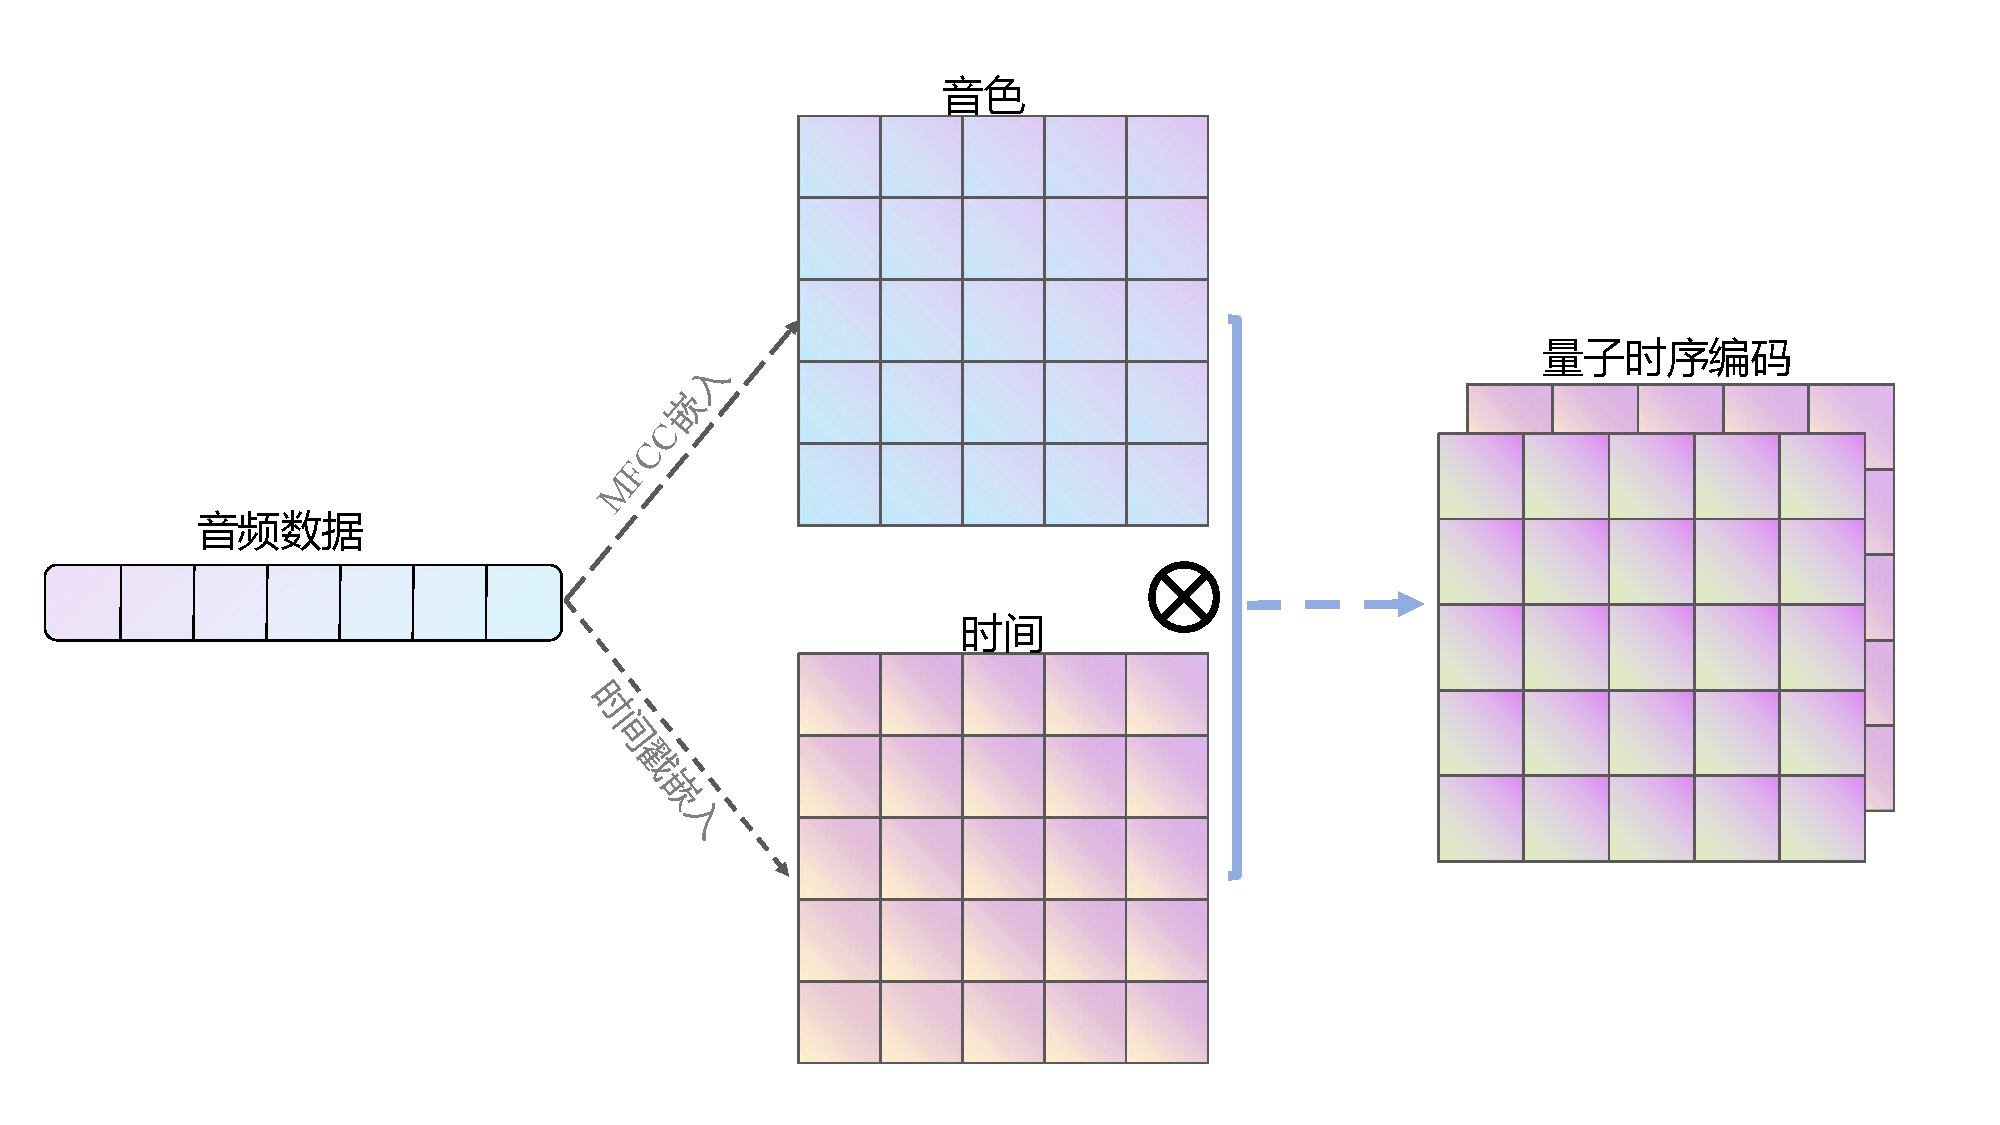
\includegraphics[width=\textwidth]{images/The structure of QTSE.pdf}
	\caption{量子时序编码结构图}
	\label{fig:The structure of QTSE}
\end{figure}

在完成特征提取后，代表音色特质与时间坐标的两个组件通过张量积（$\otimes$）操作进行结构化组合。在这种架构设计下，时间信息不再是孤立存储的维度，而是作为音色特征演化的物理基底，共同映射为希尔伯特空间中的参数化量子态。这种双序列纠缠的联合编码机制，使得量子音频表示在保持量子并行优势的同时，具备了极强的时频拓扑表征能力。这种设计不仅提升了数据在量子比特中的存储密度，也从根本上解决了传统模型在处理高动态音频信号时建模精度不足的问题，为后续量子网络进行高效特征提取与分类决策奠定了稳固的理论基础。


\subsubsection{量子时序编码的数学模型}
\label{sec:qtse_math_model}

在明确了量子时序编码的核心概念与双序列结构之后，本节将对其进行严格的形式化定义，构建相应的数学模型。

假设经过特征提取与离散化处理后，音频的音色取值范围为 $2^q$。本研究采用一个长度为 $q$ 的二进制序列 $A_T^0 A_T^1 \ldots A_T^{q-2} A_T^{q-1}$ 来精确编码离散采样点 $T$ 处的对应音色值 $f(T)$，其具体的数学映射关系定义如下：
\begin{equation}
	f(T) = A_T^0 A_T^1 \ldots A_T^{q-2} A_T^{q-1}, \quad A_T^k \in \{0,1\}, \quad f(T) \in \left[0, 2^q-1\right]
	\label{eq:timbre_value}
\end{equation}

对于总长度为 $L=2^n$ 的输入量子音频信号，其时间序列信息可以由 $n$ 个量子比特的基态来精确表示：
\begin{equation}
	|T\rangle = \left|t_0 t_1 \ldots t_{n-1}\right\rangle, \quad t_i \in \{0,1\}, \quad i=0,1,\cdots,n-1
	\label{eq:time_index}
\end{equation}

在此基础上，通过将音色信息所在的量子寄存器与时间信息所在的量子寄存器进行纠缠操作，量子时序编码的完整数学模型可以表示为所有时间点及其对应音色状态的均匀叠加态：

\begin{equation}
    |A\rangle = \frac{1}{\sqrt{2^n}} \sum_{T=0}^{2^n-1} |f(T)\rangle \otimes |T\rangle = \frac{1}{\sqrt{2^n}} \sum_{T=0}^{2^n-1} \left( \bigotimes_{i=0}^{q-1} |A_{T}^{i}\rangle \right) \otimes |T\rangle
    \label{eq:qtse_state}
\end{equation}
其中，$f(T)$ 表示采样点 $T$ 处的音色特征值，$|T\rangle$ 表示与该音色特征相对应的时间位置信息。

量子时序编码与传统的量子编码模型（如仅反映单一数值的振幅编码或角度编码）存在本质区别：前者直接用量子比特序列的基态表达离散采样点处的音色值。这一方案的核心优点在于，它借助量子基态固有的正交性，在统一的希尔伯特空间内对不同音色值加以区分，不存在混淆问题。

从量子资源开销角度看，一段时间帧数为 $2^n$、音色特征离散化范围为 $2^q$ 的音频信号，量子时序编码只需 $(q+n)$ 个量子比特就能完成全局时空信息的表示。这种对数量级的空间复杂度说明量子时序编码能够以有限的量子比特资源高效编码高维音频数据，为在NISQ设备上落地部署提供了较强的可行性。

\subsubsection{量子时序编码的线路实现}
\label{sec:qtse_circuit}

在量子力学框架下处理音频，第一步是把经典音频数据映射为量子态。本节给出量子时序编码的具体制备步骤及对应的量子线路结构。

假设输入音频信号的音色取值范围为 $\left[0, 2^{q} - 1\right]$，信号长度为 $L = 2^n$。在制备初始阶段，系统需要分配 $(q+n)$ 个量子比特，并将其全部初始化为基态 $|0\rangle$。因此，量子寄存器的初始状态可以表示为：
\begin{equation}
	|\Psi\rangle_0=|0\rangle^{\otimes q+n}
	\label{eq:initial_state}
\end{equation}

量子时序编码的状态制备过程主要分为以下两个核心步骤：

（1）时间信息的构建

该步骤的逻辑与 NEQR 制备过程的初始阶段相似。在此阶段，单量子比特的恒等门（Identity gate, I）用于保持音色量子比特的当前状态不变，而哈达玛门（Hadamard gate, H）则作用于时间量子比特，使其产生每个基态出现概率均等的均匀叠加态。第一步所使用的门操作矩阵表示如下：
\begin{equation}
	I=\begin{bmatrix}
		1 & 0 \\
		0 & 1
	\end{bmatrix}, \quad H=\frac{1}{\sqrt{2}}\begin{bmatrix}
		1 & 1 \\
		1 & -1
	\end{bmatrix}
	\label{eq:gates}
\end{equation}

第一步的完整量子操作可定义为 $U_1$：
\begin{equation}
	U_1=I^{\otimes q} \otimes H^{\otimes n}
	\label{eq:u1_op}
\end{equation}

在执行 $U_1$ 变换后，代表音色信息的 $q$ 个量子比特经过 $I^{\otimes q}$ 变换保持原态，而代表时间信息的 $n$ 个量子比特经过 $H^{\otimes n}$ 变换转化为叠加态。因此，系统从初始态 $|0\rangle$ 转化为代表所有“空”音频采样点叠加的中间态 $\left|\Psi_1\right\rangle$：

\begin{equation}
	\begin{aligned}
		|\Psi\rangle_1 &= U_1\left(|\Psi\rangle_0\right) \\
		&= (I|0\rangle)^{\otimes q} \otimes(H|0\rangle)^{\otimes n} \\
		&= \frac{1}{\sqrt{2}^n}|0\rangle^{\otimes q} \otimes \sum_{T=0}^{2^n-1}|T\rangle \\
		&= \frac{1}{\sqrt{2}^n} \sum_{T=0}^{2^n-1}|0\rangle^{\otimes q} \otimes |T\rangle
	\end{aligned}
	\label{eq:psi_1}
\end{equation}

（2）音色值的设定

接下来的目标是将对应的音色特征值 $f(T)$ 编码至每个采样点 $T$ 对应的量子态中。针对每一个时间采样点 $T$，我们定义一个子操作 $U_T$：
\begin{equation}
	U_T=\left(I \otimes \sum_{j=0, j \neq T}^{2^n-1}|j\rangle\langle j|\right)+\omega_T \otimes|T\rangle\langle T|
	\label{eq:u_t}
\end{equation}
其中，$\omega_T$ 是专门用于设定采样点 $T$ 音色值的核心量子操作，它由 $q$ 个量子预言机（Quantum Oracles）组合而成：
\begin{equation}
	\omega_T=\bigotimes_{i=0}^{q-1} \omega_T^i
	\label{eq:omega_t}
\end{equation}
每一个子操作 $\omega_T^i$ 的作用规则如下：
\begin{equation}
	\omega_T^i:|0\rangle \rightarrow\left|0 \oplus A_T^i\right\rangle
	\label{eq:omega_t_i}
\end{equation}
这里 $\oplus$ 代表模2加法（XOR 操作）。公式（\ref{eq:omega_t_i}）表明：如果音频特征的二进制位 $A_T^i=1$，则 $\omega_T^i:|0\rangle \rightarrow|1\rangle$，此时该操作实质上是一个由时间量子比特作为控制位、音色量子比特作为目标位的多受控非门（n-CNOT）；反之，如果 $A_T^i=0$，则 $\omega_T^i:|0\rangle \rightarrow|0\rangle$，该操作等效于量子恒等门。因此，复合操作 $\omega_T$ 的整体作用效果为：
\begin{equation}
	\omega_T|0\rangle^{\otimes q}=\bigotimes_{i=0}^{q-1}\left(\omega_T^i|0\rangle\right)=\bigotimes_{i=0}^{q-1}\left|0 \oplus A_T^i\right\rangle=\bigotimes_{i=0}^{q-1}\left|A_T^i\right\rangle=|f(T)\rangle
	\label{eq:omega_t_effect}
\end{equation}

在施加子操作 $U_T$ 后，中间态 $\left|\Psi_1\right\rangle$ 中的第 $T$ 个时间分量的音色态将被更新：

\begin{equation}
	\begin{aligned}
		U_T\left(\left|\Psi_1\right\rangle\right) &= \frac{1}{\sqrt{2^n}} \Bigg( \sum_{j=0, j \neq T}^{2^n-1}|0\rangle^{\otimes q} \otimes |j\rangle + |f(T)\rangle \otimes |T\rangle \Bigg)
	\end{aligned}
	\label{eq:ut_psi1}
\end{equation}

通过对所有 $2^n$ 个采样点依次遍历并执行相应的子操作，即可得到第二步的总操作 $U_2$：
\begin{equation}
	U_2=\prod_{T=0}^{2^n-1} U_T
	\label{eq:u2}
\end{equation}

经过总操作 $U_2$ 后，系统演化为最终的量子时序编码量子态 $|\Psi\rangle_2$：
\begin{equation}
	\begin{aligned}
		|\Psi\rangle_2 &= U_2\left(|\Psi\rangle_1\right) \\
		&= \prod_{T=0}^{2^n-1} U_T\left(|\Psi\rangle_1\right) \\
		&= \prod_{T=0}^{2^n-1} \frac{1}{\sqrt{2}^n} \Bigg( \sum_{j=0, j \neq T}^{2^n-1}|0\rangle^{\otimes q} \otimes |j\rangle + |f(T)\rangle \otimes |T\rangle \Bigg) \\
		&= \frac{1}{\sqrt{2}^n} \sum_{T=0}^{2^n-1}|f(T)\rangle \otimes |T\rangle
	\end{aligned}
	\label{eq:psi_2}
\end{equation}

完成以上两步操作后，量子时序编码的制备过程结束。下面对该方法线路实现的时间与空间复杂度作出评估。

\textbf{定理 1}\textit{对于任意一个时间采样点 $T$，通过引入优化的量子比特复用策略，量子操作 $U_T$ 的实现复杂度不超过 $O(qn)$。}

\textbf{证明：}子操作 $U_T$ 的核心任务是把采样点 $T$ 的音色信息 $f(T)$ 写入对应的音色量子比特。该操作的主体 $\omega_T$ 利用了量子时序编码中音色量子比特兼任“存储位”与“辅助位”的双重身份，以此分解并执行多受控门。在量子时序编码的优化方案中，音色量子比特既用来最终保存音频采样值，又同时充当辅助比特，配合分解复杂的多受控门（如 n-CNOT 门）。

具体来说，对于每个采样点 $T$，需要应用受 $n$ 个时间量子比特控制、作用于 $q$ 个音色量子比特上的条件翻转操作，这总共需要 $q$ 个 n-CNOT 门。根据 NEQR 模型中关于线路复杂度的研究，当系统存在可用的辅助比特时，一个 k-CNOT 门可以被分解为 $O(k)$ 个基础的 2-CNOT 门。由于量子时序编码直接复用音色量子比特作为辅助比特，无需额外引入专用的辅助比特，因此每个 n-CNOT 门的分解复杂度维持在 $O(n)$。综上所述，执行单个 $U_T$ 组合操作的时间复杂度为 $O(q \cdot n) = O(qn)$。

\textbf{引理 1}\textit{在量子时序编码的制备线路之中，第二步操作的总时间复杂度为 $O\left(q n 2^n\right)$。}

\textbf{证明：}根据定理 1，单个子操作 $U_T$ 的时间复杂度为 $O(qn)$。第二步需要对所有 $2^n$ 个采样点顺序执行这一子操作。利用上述量子比特复用策略，所有受控操作均可在不额外增加辅助比特的情况下完成。因此，第二步操作的总时间复杂度为 $2^n \cdot O(q n) = O\left(q n 2^n\right)$。

为了将抽象的数学推导与具体的网络架构对接，我们以总数为 8 个量子比特的系统为例（其中音色编码分配 $q = 4$ 个量子比特，时间编码分配 $n = 4$ 个量子比特）。从经典 MFCC 特征到量子态的映射步骤如下：
（1）提取音频每一帧的 $D$ 维 MFCC 特征向量；
（2）将整段音频信号分割为 $2^n = 16$ 帧，对应的时间索引为 $T \in [0, 15]$；
（3）通过归一化与均匀分箱操作，将每一帧的 $D$ 维 MFCC 向量压缩为一个标量音色值 $f(T) \in [0, 15]$，并将其表示为 4 位二进制字符串 $A_T^3 A_T^2 A_T^1 A_T^0$；
（4）按照上述两步制备流程，将这 16 个“音色-时间”映射对编码进入量子态。

\begin{figure}[!htb]
	\centering
	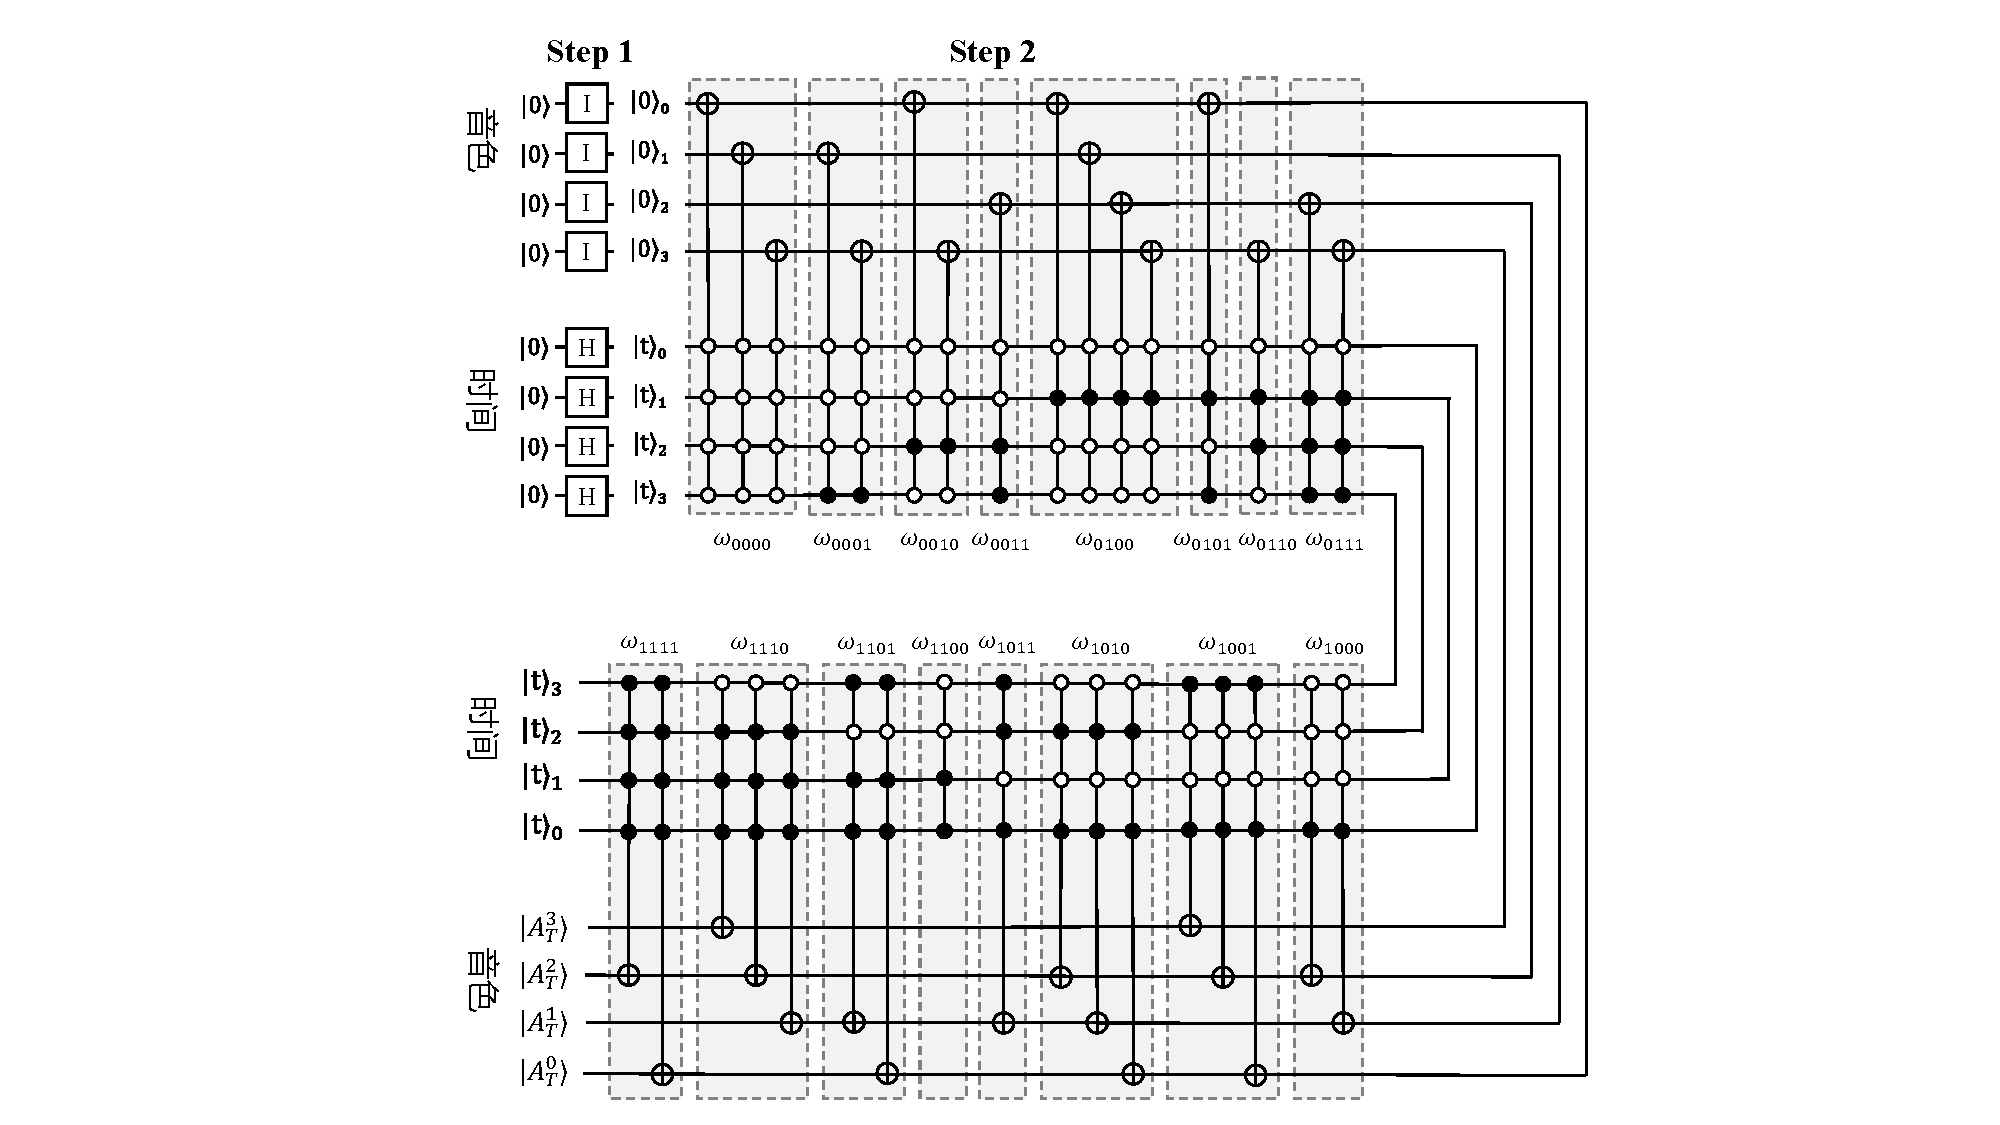
\includegraphics[width=\textwidth]{images/Quantum circuit for QTSE preparation for the audio.pdf}
	\caption{量子时序编码制备量子线路图（以 $n=4$, $q=4$ 为例）。其中，第一步利用哈达玛门初始化时间序列的叠加态；第二步通过 16 个子操作（$\omega_{0000}$ 至 $\omega_{1111}$）编码音色值，每个子操作均使用多受控非门。图中的实心圆代表控制条件为 $|1\rangle$，空心圆代表控制条件为 $|0\rangle$。}
	\label{fig: Quantum circuit for QTSE preparation for the audio}
\end{figure}


如图~\ref{fig: Quantum circuit for QTSE preparation for the audio} 展示的 $n=4, q=4$ 情况下的具体实现，第二步由 $2^n=16$ 个子模块（如 $\omega_T$）构成。每个子模块均采用多受控非门机制：以 $n$ 个时间量子比特为控制节点，当其序列处于特定态（如 $|0001\rangle$）时，该模块被激活，并根据离散特征值 $f(T)$ 的二进制编码对 $q$ 个音色量子比特执行受控翻转。尽管理论上该步骤需要 $O(q n 2^n)$ 个逻辑门，但在实际映射中，大量的零位对应恒等操作，从而在实践中有效降低了线路的深度。


\textbf{定理 2}\textit{针对长度为 $2^n$ 且音色取值范围为 $2^q$ 的音频信号，量子时序编码的整体制备时间复杂度为 $O\left(q n 2^n\right)$，且总共仅需占用 $q+n$ 个量子比特。相较于传统编码方法，量子时序编码通过借鉴 NEQR 的基态表示逻辑实现了资源优化。}

\textbf{证明：} 将第一步操作的时间复杂度 $O(q+n)$ 与第二步操作的时间复杂度 $O\left(q n 2^n\right)$ 合并后，量子时序编码的全局时间复杂度为：$O(q+n) + O\left(q n 2^n\right) = O\left(q n 2^n\right)$。在空间复杂度方面，由于采用双比特序列纠缠映射，系统仅需占用 $q+n$ 个量子比特即可完成全局信息的表征。综合来看，该方案在保证时频特征高保真映射的前提下，有效控制了线路深度与量子比特开销，在 NISQ 设备及工程部署层面表现出良好的适用性。

\subsection{量子时频分析神经网络模型}
\label{sec:qann_model}

量子时频分析神经网络是一种端到端的量子神经网络架构，将经典深度学习中分层提取特征的思路与量子叠加态、纠缠态的物理性质相结合\citess{henderson2020quanvolutional,cong2019quantum}。该架构形成了一条完整的量子信息处理流水线，从特征编码到分类预测均在同一框架内完成。网络整体包含五个组件：量子数据编码模块（即前述量子时序编码器）、量子卷积层、量子池化层、量子全连接层和量子测量模块。

\begin{figure}[!htb]
	\centering
	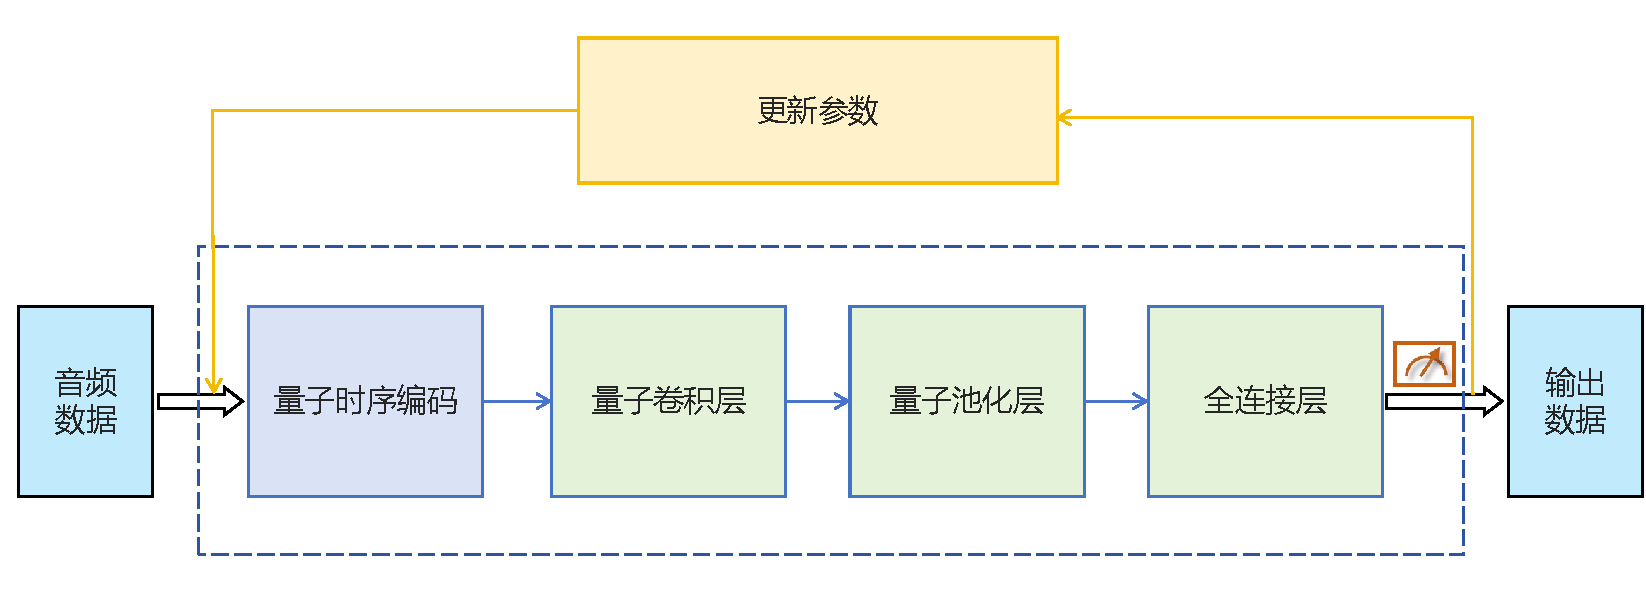
\includegraphics[width=1.0\textwidth]{images/The structure of QANN.pdf}
	\caption{量子时频分析神经网络整体结构框架图}
	\label{fig:The structure of QANN}
\end{figure}

如图~\ref{fig:The structure of QANN} 所示，量子时频分析神经网络的流水线处理遵循一个清晰且连贯的数据流。整个处理过程首先从原始音频数据开始，通过预处理提取出经典的梅尔频率倒谱系数特征。随后，这些经典的时序特征数据被送入量子时序编码模块，转换为高维希尔伯特空间中的量子态。这一步骤完成了经典信息向量子信息的跨越。该量子态作为初始状态被输入到由交替排列的量子卷积层和量子池化层构成的核心处理线路中。经过特征提取与全连接层降维后，系统通过测量模块对输出量子比特执行投影测量，将处理后的量子态映射回经典概率域，输出最终预测结果。

如图~\ref{fig:The circuit of QANN} 所示，量子时频分析神经网络的核心量子线路实现了上述处理流程。量子时序编码作为编码层已在本章 3.1 节中讨论。本文的量子演化线路在设计上遵循了硬件高效拟设的原则，这对于模型在 NISQ 设备上的实际运行至关重要。线路深度被有意控制在较浅的水平，旨在减轻硬件噪声的干扰并有效抑制大规模变分线路中常见的“贫瘠高原”现象。

\begin{figure}[!htb]
	\centering
	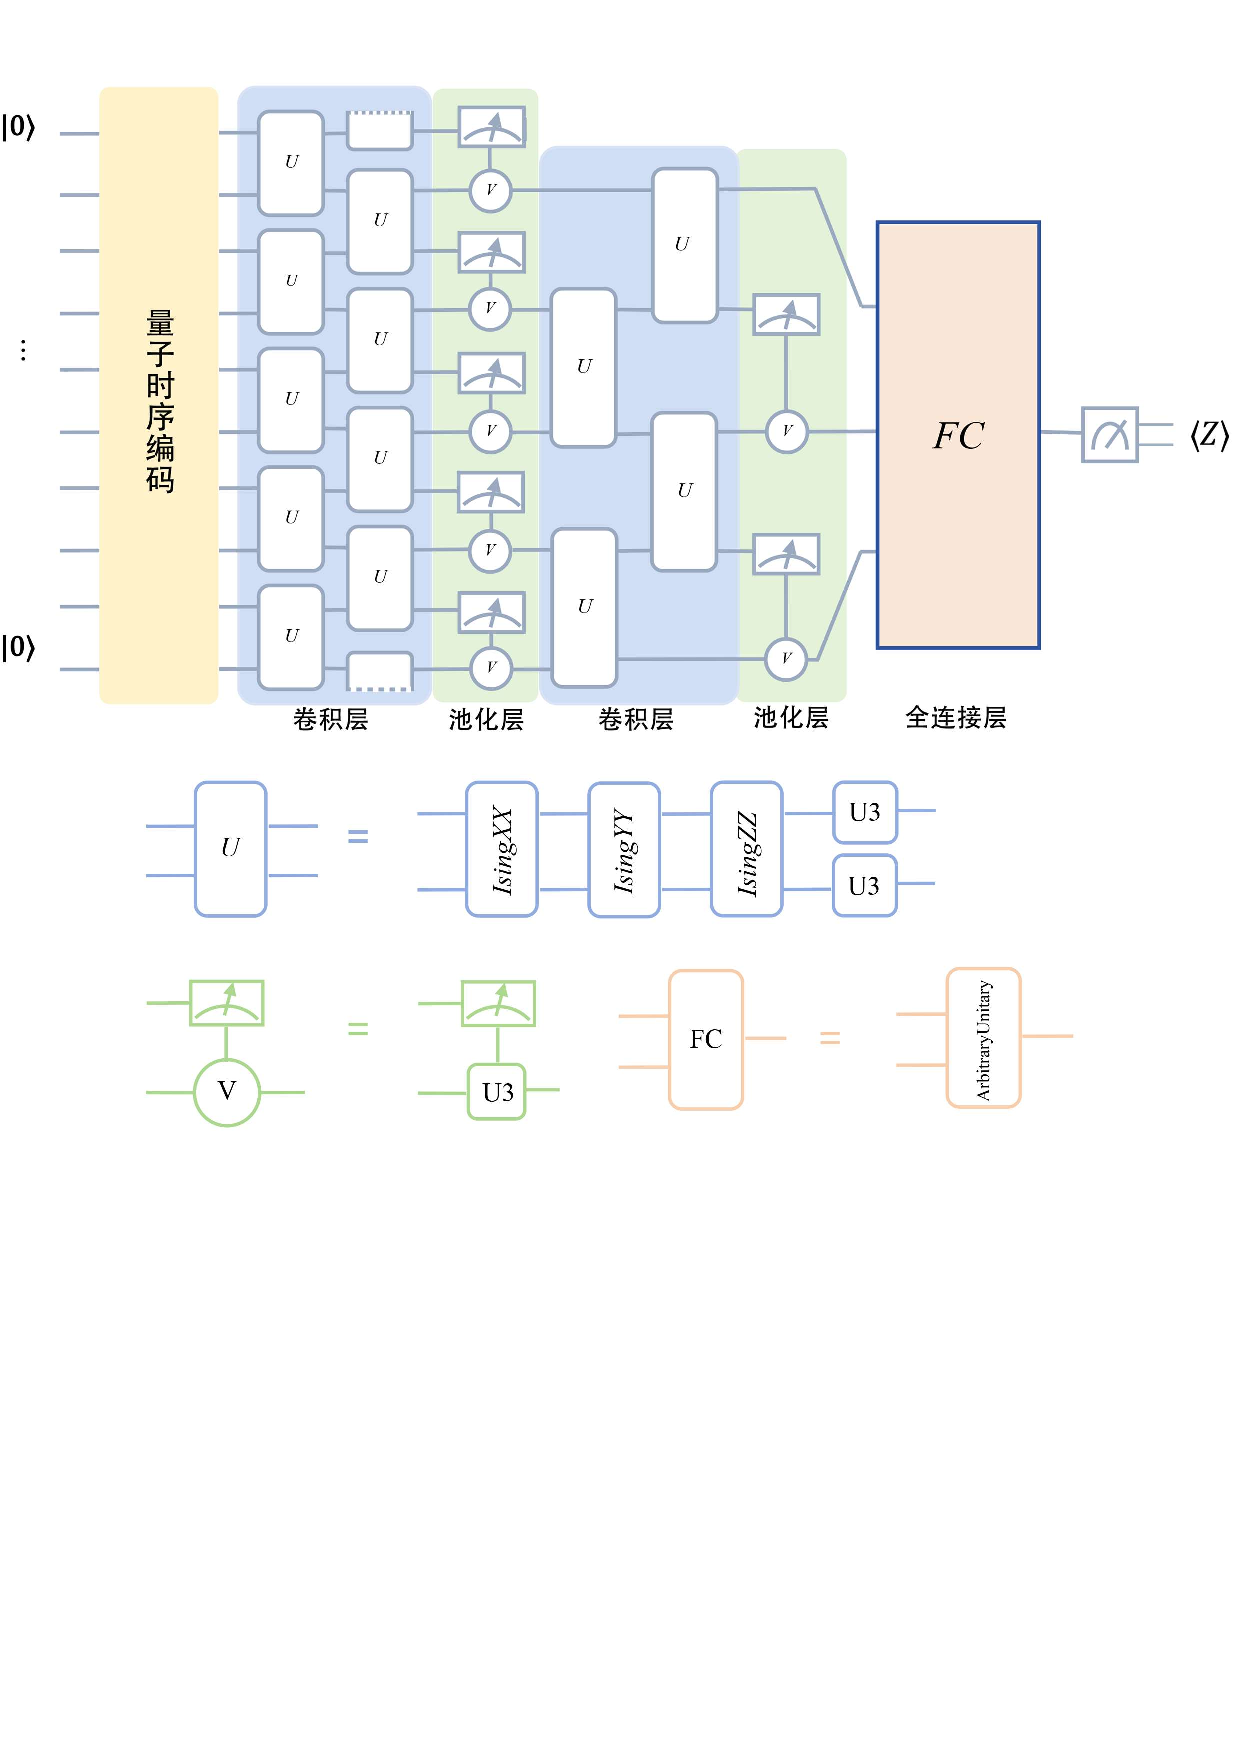
\includegraphics[width=1.0\textwidth]{images/The circuit of QANN.pdf}
	\caption{量子时频分析神经网络核心线路结构图}
	\label{fig:The circuit of QANN}
\end{figure}

\subsubsection{量子卷积层}
\label{subsec:q_conv}

量子卷积层扮演局部特征提取器的角色，用于捕获量子比特上相邻音频特征数据点间的关联。在经典深度学习中，卷积神经网络通过固定大小的卷积核在输入数据上滑动来提取局部空间特征；而在量子范式下，这一过程被重新诠释为参数化酉变换在相邻量子比特对上的平移施加。量子卷积层的核心是参数化量子滤波器 $U$，其门电路的组合方式对经典卷积核的模拟至为关键，由以下两部分构成：

（1）U3 门：作为通用单量子比特旋转门，U3 门可以实现布洛赫球面上的任意单量子比特旋转操作，是主要的可学习参数载体。其矩阵形式为：
\begin{equation}
	U_3(\theta, \phi, \lambda) = \begin{bmatrix}
		\cos\frac{\theta}{2} & -e^{i\lambda}\sin\frac{\theta}{2} \\
		e^{i\phi}\sin\frac{\theta}{2} & e^{i(\phi+\lambda)}\cos\frac{\theta}{2}
	\end{bmatrix}
	\label{eq:u3_gate}
\end{equation}
其中 $\theta$ 控制绕 Y 轴的旋转幅度，$\phi$ 和 $\lambda$ 分别控制绕 Z 轴的旋转相位。三个连续参数赋予了 U3 门覆盖整个 $SU(2)$ 群的能力，使其能够为滤波器提供在单个量子比特上拟合复杂变换所需要的表达空间。

（2）伊辛族门（Ising-family Gates: XX, YY, ZZ）：这些双量子比特门被专门选用以在相邻量子比特之间生成纠缠。其中，$\text{Ising}XX(\alpha) = \exp\left(-i \frac{\alpha}{2} X \otimes X\right)$ 在 X 基上耦合两个量子比特的自旋，$\text{Ising}YY(\beta) = \exp\left(-i \frac{\beta}{2} Y \otimes Y\right)$ 和 $\text{Ising}ZZ(\gamma) = \exp\left(-i \frac{\gamma}{2} Z \otimes Z\right)$ 分别在 Y 基和 Z 基上完成类似操作。三种伊辛门的级联等效于在三个正交的泡利基方向上施加独立的相互作用强度，使双比特纠缠结构具备各向异性的调控自由度。这一功能对于建模相邻时频特征之间的局部相关性至关重要，从而再现了经典卷积中的“局部感受野”概念。

在数学上，量子卷积操作可以表示为：
\begin{equation}
	U = U_3\left(\theta_1, \phi_1, \lambda_1\right) \otimes U_3\left(\theta_2, \phi_2, \lambda_2\right) \cdot \text{Ising}ZZ(\gamma) \cdot \text{Ising}YY(\beta) \cdot \text{Ising}XX(\alpha)
	\label{eq:q_conv}
\end{equation}
其中 $\alpha, \beta, \gamma, \theta_1, \phi_1, \lambda_1, \theta_2, \phi_2, \lambda_2$ 共计 9 个可训练参数。从结构上看，伊辛族门首先在底层建立两个量子比特的纠缠关联，随后各自独立的 U3 门对已纠缠的量子态做进一步的局部旋转。这一“先纠缠、后旋转”的流水线设计保证了滤波器既能够学习两个时频通道之间的关联模式，又能在各通道内独立调整振幅与相位。

同一层内所有 $U$ 滤波器共用公式（\ref{eq:q_conv}）中的这组参数。这一参数共享策略直接类比于经典卷积中同一卷积核在不同空间位置共享权重的做法。其物理含义在于：无论音频特征出现在哪个时间帧位置，模型都使用相同的量子变换去检测该特征，由此保证了声学模式识别的平移不变性。这一设计不仅为生成具有平移不变性的特征图提供了基础，也使模型的参数总量得到有效压缩——相较于为每对量子比特分配独立参数的全参数化方案，参数共享使卷积层的参数量从 $O(9N)$ 降低至固定的 9 个，其中 $N$ 为量子比特对的数目。

在量子卷积层的实际运行中，参数化滤波器 $U$ 以步长为 1 的方式在相邻量子比特对上滑动。假设输入态包含 $N$ 个量子比特，则滤波器依次作用于
$(q_0, q_1)$, $(q_1, q_2)$, $\ldots$, $(q_{N-2}, q_{N-1})$
共 $N-1$ 个量子比特对，每次施加相同的酉变换 $U$。整个量子卷积层的复合操作 $U_{\text{conv}}$ 可写为：
\begin{equation}
	U_{\text{conv}} = \prod_{k=0}^{N-2} U^{(k, k+1)}
	\label{eq:q_conv_total}
\end{equation}
其中 $U^{(k, k+1)}$ 表示作用在第 $k$ 与第 $k+1$ 个量子比特上的参数化滤波器。该操作完成后，量子态中蕴含的局部时频关联被逐步提取并编码到纠缠度更高的全局特征态中，为后续的池化与分类步骤提供信息基础。

\subsubsection{量子池化层}
\label{subsec:q_pool}

量子池化层承担特征聚合与降维的工作，有助于减小模型复杂度以及后续层所需的量子比特数。在经典卷积神经网络中，池化操作（如最大池化或平均池化）通过在局部窗口内选取代表性数值来实现空间维度的缩减；而在量子范式下，由于量子不可克隆定理的约束，不可能直接复制和比较量子态，因此需要一种与经典方法本质不同的信息压缩机制。量子池化层正是为满足这一需求而设计的：它通过量子门操作与部分量子比特的丢弃，将多个量子比特上的特征信息压缩到更少的量子比特中，同时尽可能保留对分类任务至关重要的特征关联。

该层以受控 U3 门为基本单元：接收两个相邻量子比特作为输入，输出一个压缩后的量子比特态。受控 U3 门是一种双量子比特门，当且仅当控制量子比特处于 $|1\rangle$ 态时，才对目标量子比特施加 U3 旋转变换。其酉矩阵在双比特计算基下的表示为：
\begin{equation}
	CU_3(\theta, \phi, \lambda) = |0\rangle\langle 0| \otimes I + |1\rangle\langle 1| \otimes U_3(\theta, \phi, \lambda)
	\label{eq:cu3_gate}
\end{equation}
其中 $I$ 为 $2 \times 2$ 的单位矩阵，$U_3(\theta, \phi, \lambda)$ 的定义如公式（\ref{eq:u3_gate}）所示。

在操作过程中，第一个量子比特（控制位）的量子态决定是否对第二个量子比特（目标位）施加参数化旋转变换。当控制位的量子态为 $|0\rangle$ 和 $|1\rangle$ 的叠加态时，目标位将处于“既被变换又未被变换”的量子叠加之中，由此实现条件压缩。与经典池化不同，这里借助量子测量的概率特性引入非线性，同时纠缠结构有助于保留更多的特征信息。数学形式如下：
\begin{equation}
	V = U_3(\phi, \theta, \lambda) \quad \text{（受相邻量子比特状态控制）}
	\label{eq:q_pool}
\end{equation}
其中 $\phi, \theta, \lambda$ 为该层的 3 个可训练参数。

假设池化前系统有 $N$ 个量子比特。池化层将这些量子比特两两配对为 $(q_0, q_1))$, $(q_2, q_3), \ldots, (q_{N-2}, q_{N-1})$，在每一对中以第一个量子比特为控制位、第二个量子比特为目标位施加受控 U3 门，随后丢弃控制位量子比特。整个池化操作可形式化表示为：
\begin{equation}
	U_{\text{pool}} = \prod_{k=0}^{N/2-1} CU_3^{(2k, 2k+1)}(\theta, \phi, \lambda)
	\label{eq:q_pool_total}
\end{equation}
经该操作后，系统的有效量子比特数从 $N$ 减半为 $N/2$，被保留的目标位量子比特携带了原先两个量子比特的压缩特征信息。

这一降维机制在信息论意义上具有独特优势。经典的最大池化或平均池化是确定性操作，固定地选取局部最大值或均值，丢弃所有其他信息；而量子池化通过受控酉变换将控制位的特征信息有条件地转移至目标位，信息的保留与丢弃比例由可训练参数 $(\theta, \phi, \lambda)$ 在训练过程中自适应决定。因此，量子池化层能够在降低维度的同时，学习到一种对分类目标最优的特征聚合策略，而非像经典池化那样采用固定的聚合规则。

此外，量子池化层在抑制过拟合方面也发挥着正则化作用。每经过一次池化操作，参与后续计算的量子比特数减半，这直接缩小了后续参数化层所能作用的希尔伯特空间维度，从而限制了模型的有效容量。这种结构化的维度递减效应类似于经典网络中池化层对过拟合的天然抑制作用，对于仅拥有 33 个可训练参数的轻量化量子网络而言，有助于在有限的训练数据条件下维持稳健的泛化性能。

\subsubsection{量子全连接层}
\label{subsec:q_fc}

量子全连接层的作用是把低维特征投射到高维类别空间，位于量子卷积层与池化层之后、测量模块之前，承担着全局特征整合与类别映射的关键角色。在经典深度学习中，全连接层通过权重矩阵将上一层的所有神经元输出线性组合并映射至类别维度；在量子范式下，这一过程由作用于所有保留量子比特的全局参数化酉变换来实现。

该层通过一系列参数化量子门的级联来实现任意酉变换，从而捕获特征之间的全局关联。经过卷积层和池化层的逐层处理后，系统中保留下来的量子比特已经编码了高度抽象的局部时频特征。然而，现有方法尚未充分挖掘这些特征间潜在的长程相关性，特别是不同频段间的谐波共振以及跨时间帧的节奏规律。量子全连接层通过在所有保留量子比特之间建立全局纠缠，打破了卷积层中局部感受野的限制，使模型能够综合利用分布在不同量子比特上的互补信息来构建最终的分类决策边界。

量子全连接层由 $L$ 层参数化酉变换级联而成。每一层 $U_i(\theta_i)$ 包含两个子步骤：首先，对每个量子比特独立施加单比特旋转门（如 $R_Y$ 或 U3 门）以引入局部参数自由度；随后，通过双比特纠缠门（如 CNOT 门或 CZ 门）在所有量子比特对之间建立全连接的纠缠结构。其中单层变换 $U_i$ 的结构可表示为：
\begin{equation}
	U_i(\theta_i) = \left(\prod_{\langle j,k \rangle} \text{CNOT}^{(j,k)}\right) \cdot \left(\bigotimes_{j=1}^{M} R_Y^{(j)}(\theta_i^{(j)})\right)
	\label{eq:q_fc_layer}
\end{equation}
其中 $M$ 为池化后保留的量子比特数目，$\langle j,k \rangle$ 遍历所有需要纠缠的量子比特对，$\theta_i^{(j)}$ 为第 $i$ 层第 $j$ 个量子比特的旋转参数。

该层展现出明显的物理与计算特性。$M$ 个量子比特构成的希尔伯特空间维度随比特数呈指数增长，使得全连接层能够在一个 $2^M$ 维的复向量空间中执行特征变换，从而以极小的参数开销捕获经典网络难以建模的高维非线性关联。参数化方案在维持高表达力的同时大幅削减了权重量，且量子叠加特性允许模型在计算过程中利用量子并行性，提升了处理复杂映射的效率。其数学表示为：
\begin{equation}
	FC = \prod_{i=1}^L U_i\left(\theta_i\right)
	\label{eq:q_fc}
\end{equation}
其中 $L$ 为该层的深度，$\theta_i$ 表示每一层对应的参数向量。

从表达能力的角度来看，量子全连接层的多层级联结构赋予了它逼近任意酉变换的理论能力。根据量子线路的普适性定理，任意 $n$ 量子比特上的酉变换都可以被分解为单比特旋转门与双比特 CNOT 门的有限组合。当级联深度 $L$ 足够大时，$FC = \prod_{i=1}^L U_i(\theta_i)$ 能够以任意精度逼近 $2^M \times 2^M$ 酉群 $SU(2^M)$ 中的任意元素，其中 $M$ 为量子比特数。这意味着量子全连接层理论上可以实现从特征空间到类别空间的任意映射，其表达能力远超参数规模相同的经典全连接层。

在本文的量子时频分析神经网络中，经过一轮卷积-池化操作后，8 个量子比特被压缩为 4 个。量子全连接层作用于这 4 个量子比特，其对应的希尔伯特空间维度为 $2^4 = 16$，即全连接层在一个 16 维的复向量空间中进行全局特征变换。这一维度对于二分类任务而言提供了充足的表达空间，同时保持了线路深度的可控性。全连接层的参数总数为 $L \times M$（每层 $M$ 个旋转参数），在本文的配置中约为 12 至 16 个参数，占网络 33 个总参数的较大比重，体现了该层在整个网络中承担主要决策功能的角色。

值得指出的是，量子全连接层的设计需要在表达能力与训练可行性之间取得平衡。过深的级联层数 $L$ 虽然提升了酉群覆盖能力，但也增加了量子线路深度，可能在 NISQ 设备上引发更多退相干噪声，并增大梯度消失风险。本文通过控制全连接层深度 $L$ 在较小范围内，并配合硬件高效拟设原则选择纠缠拓扑，在保证分类精度的前提下将线路深度维持在 NISQ 设备可接受的水平。

\subsubsection{量子测量模块}
\label{subsec:q_measure}

测量模块充当量子处理单元与经典输出之间的桥梁，将末态量子信号转换为可用于分类的经典概率分布。在量子时频分析神经网络的末端，系统在泡利-Z 基（Pauli-Z basis）上执行投影测量以获取经典读数。该操作把量子态投影至基态，完成从叠加态到经典概率的映射。测量过程可写为：
\begin{equation}
	E = \left\langle\phi\right|_{in} \left(F(\theta_3)V(\theta_2)U(\theta_1)\right)^* Z \left(F(\theta_3)V(\theta_2)U(\theta_1)\right) \left|\phi\right\rangle_{in}
	\label{eq:q_measure}
\end{equation}
其中 $F, V, U$ 分别代表全连接层、池化层和卷积层的变换映射，$\theta_3, \theta_2, \theta_1$ 为对应各层的可训练参数集合，$Z$ 为 Pauli-Z 测量算符。

经由上述测量，量子时频分析神经网络完成了从量子特征到分类结果的完整转换。在实际模拟中，期望值 $E$ 通过多次重复测量来统计估计，随后映射为音频分类所需的经典概率。

为更清楚地展示该架构的数据流向与计算逻辑，表 \ref{alg:forward_propagation} 归纳了基于时序编码的量子时频分析神经网络前向传播算法的各个步骤，覆盖了从经典音频特征输入、量子态制备、变分线路演化直到概率输出的全过程。

\begin{table}[!htb]
	\centering
	\caption{量子时频分析神经网络前向传播与分类算法}
	\label{alg:forward_propagation}
	\renewcommand{\arraystretch}{1.3} % 调整行高，使表格排版更舒展
	\begin{tabular}{p{0.95\textwidth}}
		\toprule
		\textbf{算法 3-1} 量子时频分析神经网络前向传播与分类算法 \\
		\midrule
		\textbf{Require:} 经典音频信号样本 $x$、量子线路的层数配置参数、量子时频分析神经网络的可训练参数集合 $\Theta = \{\theta_1, \theta_2, \theta_3\}$、测量的观测算符（Pauli-Z）； \\
		\textbf{Ensure:} 目标音频的类别预测概率分布 $P(y|x)$； \\
		\textbf{Step 1 经典预处理：} 对输入音频信号 $x$ 执行分帧与加窗操作，提取梅尔频率倒谱系数特征序列，并将其离散化为音色值 $f(T)$ 与对应的时间索引 $T$； \\
		\textbf{Step 2 量子时序编码：} 初始化 $(q+n)$ 个量子比特为 $|0\rangle^{\otimes q+n}$ 态； \\
		\textbf{Step 3：} 对时间量子比特施加哈达玛门生成均匀叠加态，并利用多受控非门将音色值 $f(T)$ 纠缠至对应的时序基态上，制备出初始量子态 $|\psi\rangle_{in}$； \\
		\textbf{Step 4 量子卷积层演化：} 将初始态输入参数化量子滤波器，通过单比特旋转门（U3）引入权重参数 $\theta_1$，利用伊辛族双比特门（XX, YY, ZZ）建立相邻时频特征的局部纠缠，输出特征态 $|\psi\rangle_{conv}$； \\
		\textbf{Step 5 量子池化层降维：} 对 $|\psi\rangle_{conv}$ 执行受控 U3 门操作（参数为 $\theta_2$），根据相邻量子比特的测量概率进行非线性压缩，抛弃冗余比特，输出降维态 $|\psi\rangle_{pool}$； \\
		\textbf{Step 6 量子全连接层映射：} 对保留下来的量子比特执行全局参数化酉变换（参数为 $\theta_3$），在整个希尔伯特空间中捕获全局特征关系，生成最终的待测量子态 $|\psi\rangle_{out}$； \\
		\textbf{Step 7 量子测量与输出：} 对网络末端的特定分类量子比特执行 Pauli-Z 投影测量； \\
		\textbf{Step 8：} 多次重复采样（Shots）以逼近该可观测量的统计期望值 $E = \langle\psi|_{out} Z |\psi\rangle_{out}$； \\
		\textbf{Step 9 经典后处理：} 将获取的连续期望值通过线性变换与激活函数映射至 $[0, 1]$ 区间，生成最终的分类预测概率分布 $P(y|x)$； \\
		\textbf{输出结果：} 输出分类概率分布 $P(y|x)$，作为模型单次前向传播的最终推理结果。 \\
		\bottomrule
	\end{tabular}
\end{table}

\subsection{实验结果与对比分析}
\label{sec:experiment_and_discussion}

本节基于 GTZAN 数据集，对量子时频分析神经网络及量子时序编码方法展开多维度的性能评估。实验详细对比了本模型在不同编码范式下，以及与基准模型（QCNN、经典 CNN）之间的分类优势与收敛特性。此外，通过时间滞后敏感性分析与结构消融实验，进一步验证了所提网络架构在捕获音频动态时序特征方面的有效性与结构必要性。

\subsubsection{实验环境与数据集}
\label{subsec:experimental_setup}

本研究的量子模拟实验均基于 PennyLane 量子机器学习框架搭建。PennyLane 是由 Xanadu 公司开发的开源量子机器学习框架，专为变分量子线路的自动微分与经典-量子混合计算设计。其核心机制包括：量子节点（QNode）、支持参数平移规则的自动微分引擎，以及多硬件后端抽象。结合本文所提的量子时频分析神经网络，其在该框架上的具体实现方式如下：系统利用 PennyLane 的 QNode 将前置的“量子时序编码”模块与“量子卷积层、池化层、全连接层”封装为统一的可微计算节点。在每次前向传播中，经典的 MFCC 时频特征通过参数接口传入该节点完成量子态制备，随后经过包含 33 个可训练参数的变分线路演化，并在末端调用 \texttt{qml.expval(qml.PauliZ())} 获取特定分类量子比特的期望值。在训练阶段，该量子节点被无缝集成至 PyTorch 等经典自动微分计算图中，依靠 PennyLane 的参数平移规则精确计算损失函数对这 33 个量子参数的梯度，最后交由 Adam 优化器完成参数更新。这种实现方式打通了经典特征输入到量子线路演化的端到端训练闭环，本章图3-5中测试集与训练集高度一致且平稳的收敛曲线，也从实验角度有力支撑并自证了该混合实现在框架底层的可行性与稳定性。

评估基准选用音乐信息检索领域内广泛采用的 GTZAN 数据集。该数据集共包含 1000 个音频样本，均匀分布于 Blues、Classical、Country、Disco、Hiphop、Jazz、Metal、Pop、Reggae 和 Rock 这 10 种截然不同的音乐流派中。每种流派包含 100 个样本，单段音频时长为 30 秒，标准采样率统一设置为 22050 Hz。
考虑到在经典计算机上模拟多量子比特体系的状态演化需要消耗巨大的内存与算力（尤其是涉及高维希尔伯特空间的张量积运算），直接开展十分类任务会导致实验周期过长且资源开销过载。因此，本节的实验方案聚焦于二分类场景，即从 10 个流派中通过两两配对构建出 45 组不同的二分类任务组合。这种设计不仅有效降低了经典模拟器的资源开销，同时通过覆盖所有可能的声学边界组合，能够更加严谨、全面地验证模型在处理多样化音频特征时的泛化能力。具体而言，量子态模拟的计算开销随量子比特数呈指数增长：本研究每次二分类仅需 8 量子比特（4 个音色比特与 4 个时间比特），模拟希尔伯特空间维度为 $2^8 = 256$，单个量子卷积层中相邻量子比特间的双比特纠缠门操作共涉及 7 对量子比特，单步状态演化开销固定且可控。若直接构建十分类模型，区分 10 个类别至少需要 $\lceil\log_2 10\rceil = 4$ 个输出量子比特，总量子比特数需由 8 扩展至 12 以上，希尔伯特空间维度随之增至 $2^{12} = 4096$，约为二分类方案的 16 倍；同时，卷积层中的双比特纠缠门对数由 7 对增至 11 对，使得单步状态演化与参数化梯度计算的开销进一步放大。此外，45 组二分类任务相互独立，不存在数据依赖关系，可在多台计算节点上完全并行执行，将 $C_{10}^2 = 45$ 对分类组合的总耗时线性分摊至各节点。相比串行执行单次十分类训练，并行二分类方案在经典模拟器上具备显著的工程灵活性。综上，在现阶段经典模拟器的算力约束下，二分类方案以可控的并行开销，兼顾了评估全面性（覆盖 $C_{10}^2 = 45$ 对声学边界组合）与实验可操作性。

在数据预处理阶段，为了使经典声学特征能够适配本文设计的 8 量子比特（即张成 $2^8$ 维度的希尔伯特空间）网络架构，本研究制定了严格的降维与采样策略。在实际操作中：针对每段 30 秒的音频信号，系统沿时间轴对其进行等间隔采样，提取出连续的 16 个时间帧；随后，计算每一帧的 13 维 MFCC 向量。为了将这些特征转换为适合量子时序编码机制的输入格式，所有的 MFCC 特征均经过全局归一化处理，并进一步量化为 4-bit 的离散音色值。这种时频联合的离散化处理，在实现数据高效降维的基础上，一定程度地避免了音频关键声学细节与宏观时序特征的流失。

在网络训练参数与配置方面，本研究综合考量了量子特征表示的保真度、优化稳定度以及底层硬件约束。如表 \ref{tab:training_config} 所示，网络批大小（Batch size）设定为 8，较小的批次规模不仅有助于在训练过程中维持量子时序编码输入态的相干性，且更符合当前NISQ设备或模拟器在底层矩阵运算时的并发处理极限。训练轮数设定为 100 个迭代步数，为参数化量子线路内的旋转门与纠缠门提供了充足的寻优周期。在输出与优化端，网络直接利用 Pauli-Z 算符测量概率的期望值作为输出，选用二元交叉熵损失（BCELoss）以精确衡量概率分布与真实硬标签的差异；同时配置 Adam 优化器并将初始学习率校准为 0.001。由于参数化量子线路的损失地形往往极其复杂，这一自适应学习率配置在保障参数更新稳定性的同时，有效兼顾了整体网络的收敛速度。

\begin{table}[!htb]
	\vspace{5pt}
	\renewcommand{\arraystretch}{1.2}
	\setlength{\tabcolsep}{40pt}
	\centering
	\caption{量子时频分析神经网络训练参数配置}
	\label{tab:training_config}
	\begin{tabular}{@{}ll@{}}
		\toprule
		\textbf{参数} & \textbf{取值/配置} \\
		\midrule
		批大小 & 8 \\
		迭代轮数 & 100 \\
		激活函数 & 测量概率 \\
		量子比特数 & 8 \\
		损失函数 & BCELoss \\
		优化器 & Adam \\
		学习率 & 0.001 \\
		\bottomrule
	\end{tabular}
\end{table}

需要说明的是，受限于当前NISQ设备及经典模拟器的算力边界，本研究在实验阶段对任务进行了针对性处理。为了适应量子模拟器的计算资源限制，实验将原本的多分类任务简化为流派两两配对的二分类任务，并对特征进行了降维处理。这种处理是目前量子计算应用基础研究中为平衡模拟效率与算法验证有效性的必要权宜之计。虽然这种简化可能在一定程度上限制了模型对复杂、多类别真实音频场景的直接泛化能力，但其核心目的在于验证量子时序编码机制在底层逻辑上的可行性。


\subsubsection{模型分类性能评估}
\label{subsec:performance_analysis}

为了全面验证量子时频分析神经网络在复杂音频分类任务中的有效性，本节从四个维度展开系统的性能评估。首先，通过分析训练全周期的准确率与损失收敛曲线，剖析模型的学习稳定性与收敛动力学特征。其次，本节对比了不同量子编码范式对特征映射的影响，以验证量子时序编码在处理时序信息时的优越性。在此基础上，本节将本文模型与现有的量子卷积神经网络（QCNN）进行对比，考察两者在架构搜索成本与参数效率上的差距。最后，引入参数规模相同（仅 33 个参数）的经典 CNN 作为基线，通过准确率、精确率、召回率与 F1 分数四个维度，探讨量子网络在极低参数限制下处理非平稳信号时的表征能力与泛化优势。

（1）训练收敛性分析

根据图~\ref{fig:The accuracy and loss of QANN} 展示的收敛曲线可知，量子时频分析神经网络在 100 个迭代步内表现出稳定的学习动力学特征。在准确率演化方面，模型在初始阶段（0 至 20 步）呈现出明显的震荡，数值在 48\% 至 70\% 之间大幅波动，这反映了参数化量子线路在随机初始化后对高维参数空间的搜索与探索过程。随后在 20 至 40 步区间，准确率曲线迎来快速爬升并突破 70\% 水平，其走势总体呈明显上行趋势，中间伴随幅度递减的小幅波动，这与随机梯度优化在量子线路参数景观中的迭代搜索特点吻合。而在 40 步以后，准确率最终收敛至 75\% 附近并在此区间波动，且训练集与测试集曲线表现出极高的一致性，说明参数更新已触及当前网络容量对应的性能边界，并展现出良好的泛化稳健性。

\begin{figure}[!htb]
	\centering
	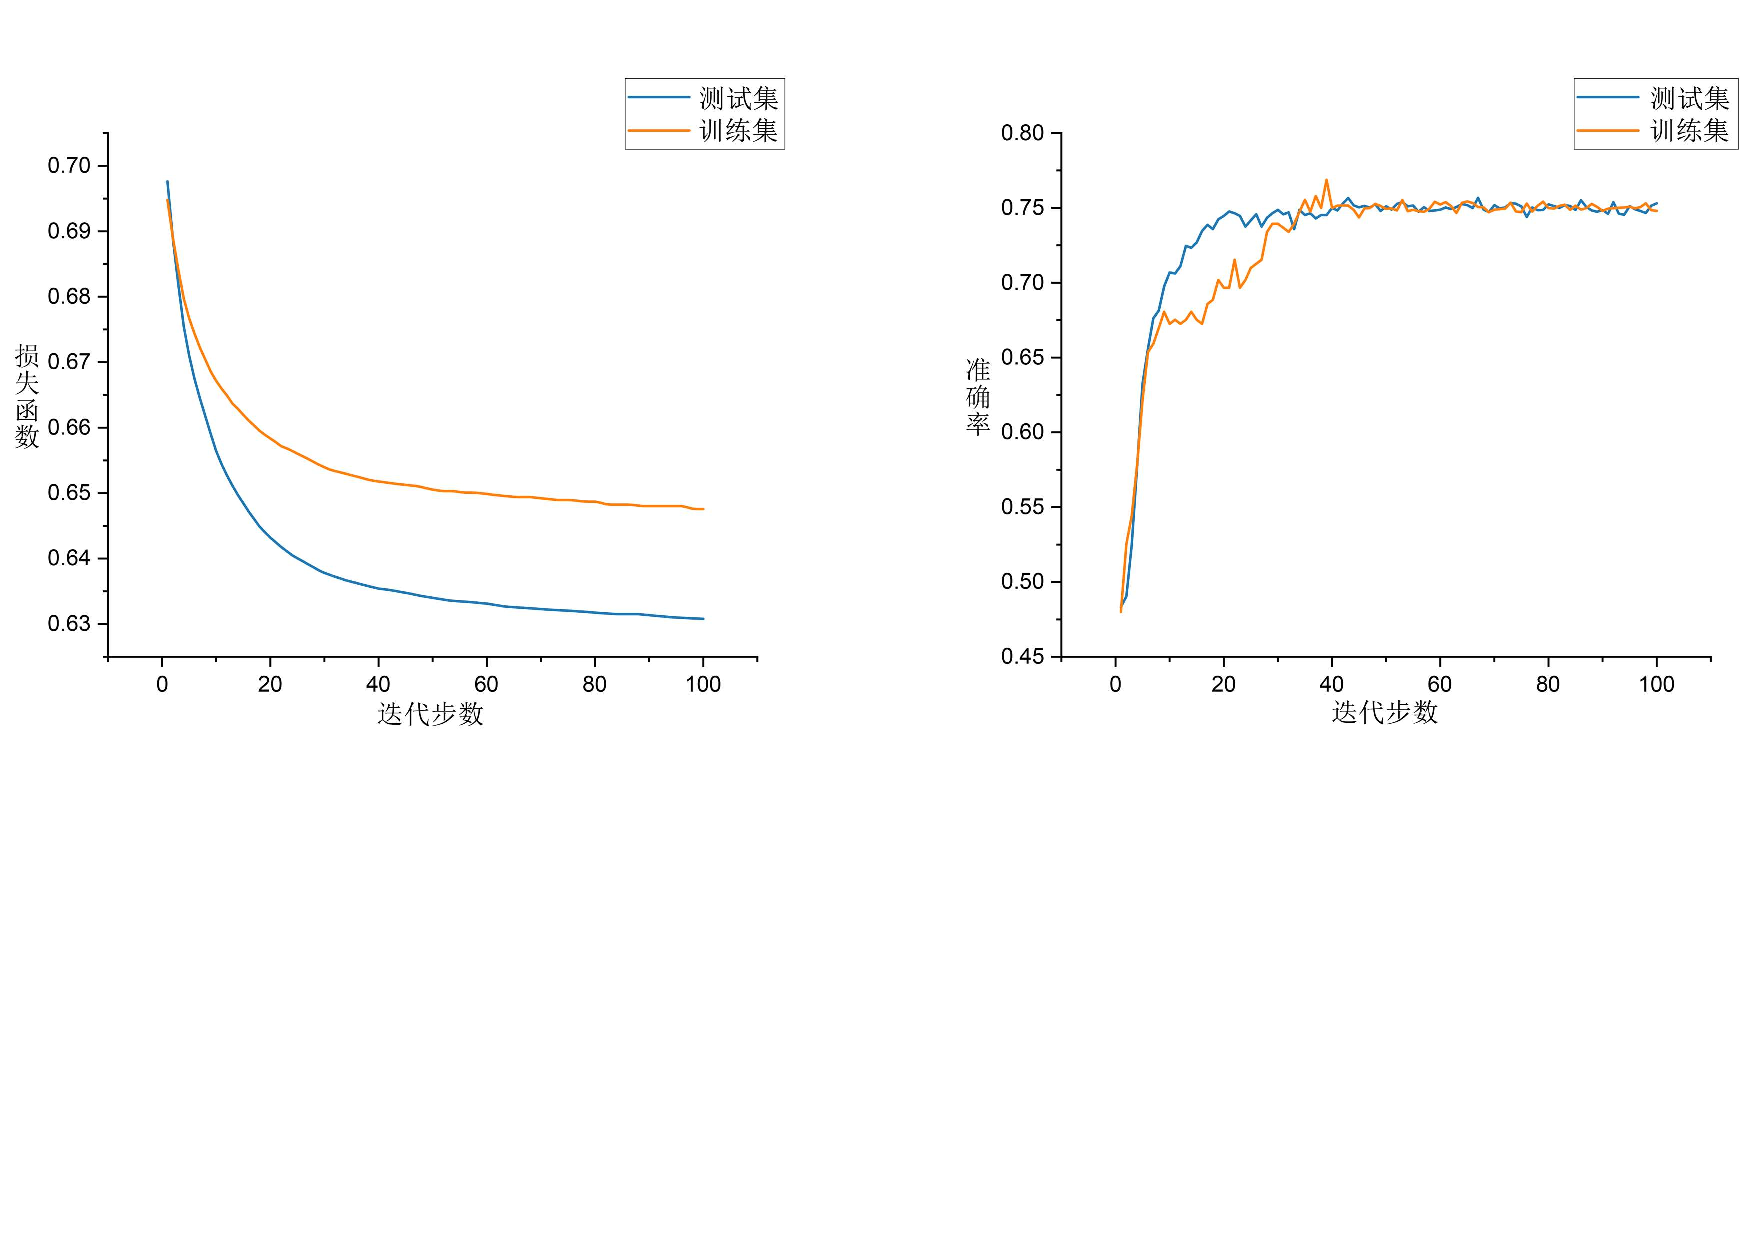
\includegraphics[width=1\textwidth]{images/The accuracy and loss of QANN.pdf}
	\caption{量子时频分析神经网络的准确率与损失收敛曲线}
	\label{fig:The accuracy and loss of QANN}
\end{figure}

损失函数曲线的走势可以与准确率对照来看，两者在时间轴上高度对齐，进一步验证了优化路径的合理性。在训练起始阶段（前 20 步），损失率在 70\% 附近起伏，对应于上述参数空间的初期探索。从第 20 到第 40 步，损失率呈现平稳下降趋势，间或出现小幅回升后继续降低的“锯齿”形态，这反映了量子参数优化过程中损失地形的复杂性。40 步之后，损失率下降至 63.5\% 至 64.5\% 之间的低位水平并趋于稳定。准确率与损失率的一致收敛说明模型训练过程稳定，参数空间的优化路径不仅实现了高效的特征捕获，也满足了 NISQ 硬件条件下的实际推理需求。

（2）不同编码方法的对比分析

如图~\ref{fig:The comparison of three encodings} 所示，本研究对比了角度编码、振幅编码与本文量子时序编码在训练过程中的分类准确率变化轨迹。从收敛速率、优化稳定性以及最终泛化精度三方面来看，不同编码范式的表现存在明显差异。

\begin{figure}[!htb]
	\centering
	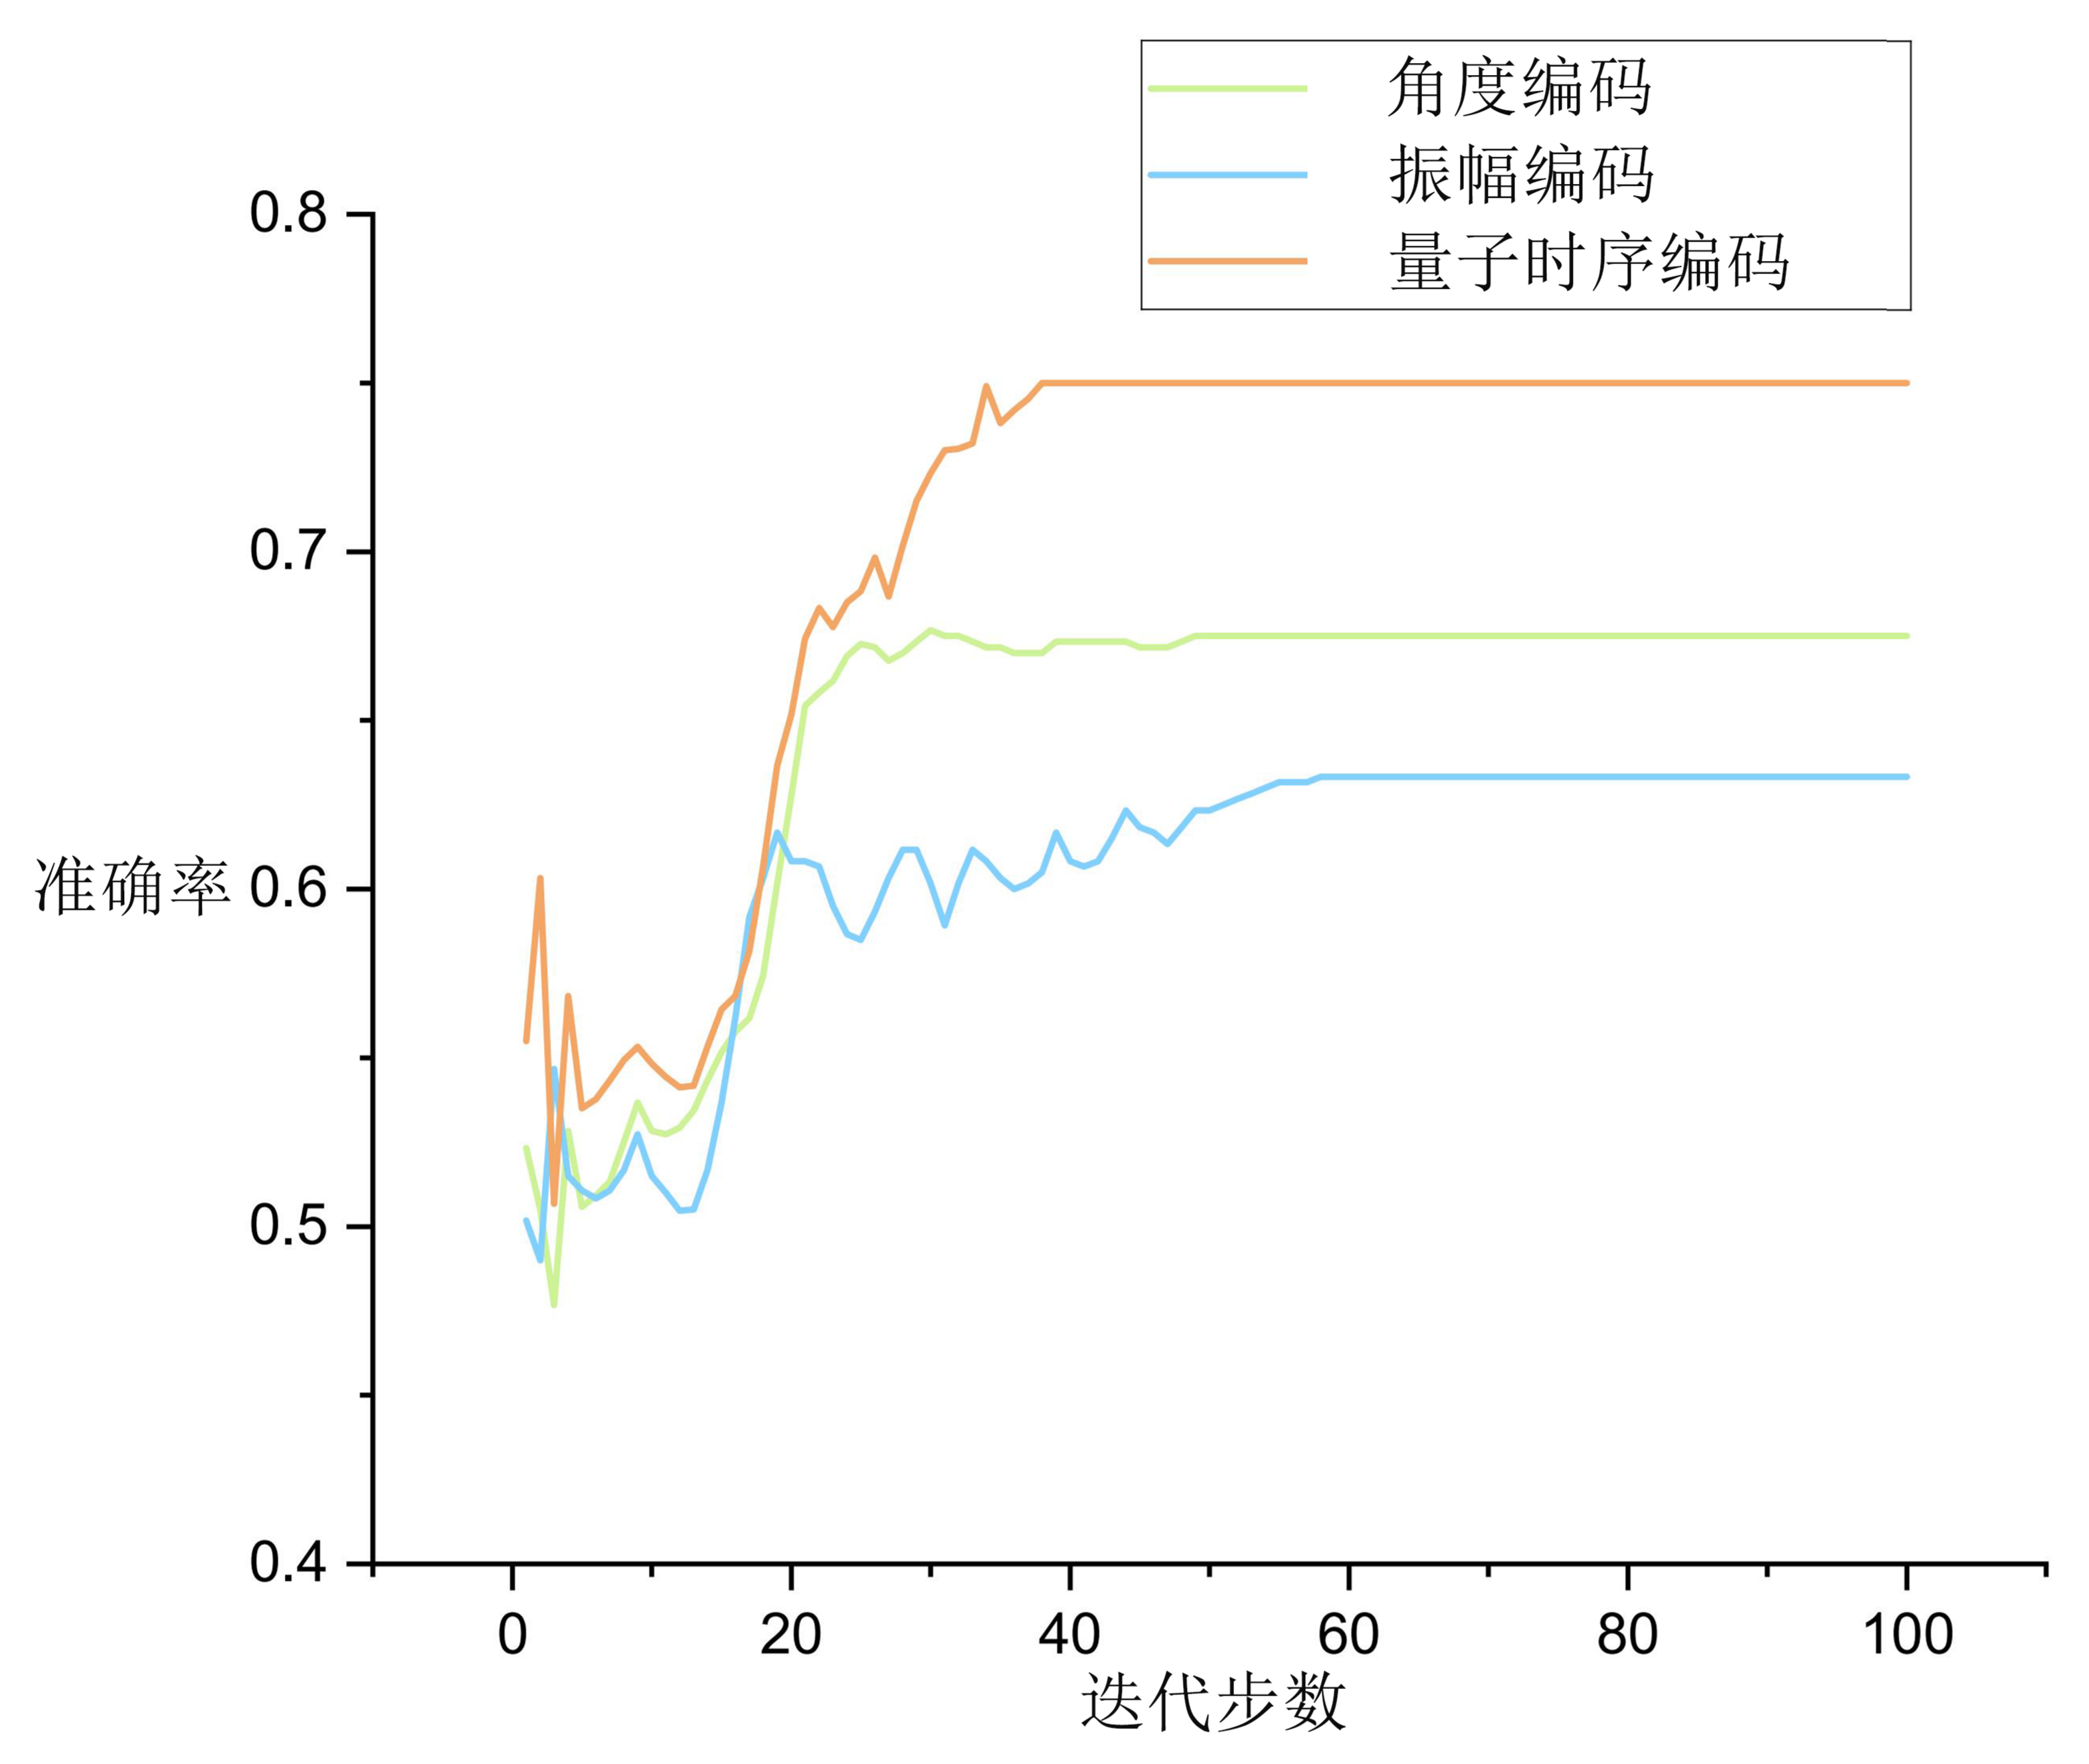
\includegraphics[width=0.6\textwidth]{images/The_comparison_of_three_encodings.png}
	\caption{不同量子编码方法的分类准确率对比}
	\label{fig:The comparison of three encodings}
\end{figure}

在训练初期（$0 \sim 20$步），三条准确率曲线均表现出不同程度的震荡，这符合参数化量子线路在非凸优化空间中进行随机搜索的物理特征。进入 20 步之后，各方案的性能表现开始显现差异：本文提出的量子时序编码（橙色曲线）展现出极高的拟合效率，准确率以较大的斜率上升，并在第 40 步附近迅速趋于平稳。相比之下，角度编码（绿色曲线）在 30 步前后即遭遇性能瓶颈，准确率上限受到明显限制；振幅编码（蓝色曲线）收敛速度最慢，且在 $20 \sim 50$步区间伴随剧烈的数值波动，直至 60 步以后才逐渐进入稳态。从收敛精度看，量子时序编码在二分类任务上的测试准确率稳定在 75\% 附近，角度编码收敛于 67\% 左右，振幅编码则渐近于 63\%。

上述性能差异的理论根源在于各编码范式对音频时序动态特征映射能力的本质区别。振幅编码虽具备指数级的状态压缩优势，但其对应的状态制备线路通常较深，极易引发“贫瘠高原”现象，导致梯度消失并限制了优化效率。角度编码虽因线路较浅而具备一定的训练稳定性，但其将音频采样帧视为相互独立的静态参数，在编码阶段便割裂了信号在时间轴上的长程上下文关联。本文提出的量子时序编码通过双比特序列机制，将离散化的 MFCC 特征与时间索引执行全局受控纠缠映射。该机制在希尔伯特空间中高保真地重构了音频信号的时频演化拓扑，使得后续的量子神经网络能够基于完备的时空关联结构构建高维决策边界，从而在收敛性能与最终精度上均实现了对传统编码方案的超越。

（3）与量子卷积神经网络的对比

本文将量子时频分析神经网络与量子卷积神经网络在 45 个音乐流派二分类任务上进行了全面对比。如图~\ref{fig:The accuracy of QANN and QCNN} 所示，从 45 个任务的总体表现来看，量子时频分析神经网络的平均准确率分布在 64.7\% 至 69.0\% 的区间内，而量子卷积神经网络的平均准确率介于 62.1\% 至 68.0\% 之间。两者约者约 2\% $\sim$ 3\% 的整体性能差距，根植于底层编码方式的不同：量子卷积神经网络依赖常规编码，输入的是降维后的 MFCC 静态统计特征，导致时间轴上的动态信息在此过程中被丢弃；而量子时频分析神经网络通过量子时序编码将含有完整时间戳的特征映射到量子纠缠态中，完整保留了音频的时空演化结构，使参数化滤波器得以精准捕获长程时间依赖。这说明量子时频分析神经网络在应对不同声学特征分布时，具备更稳定、优异的泛化性能。

\begin{figure}[!htb]
	\centering
	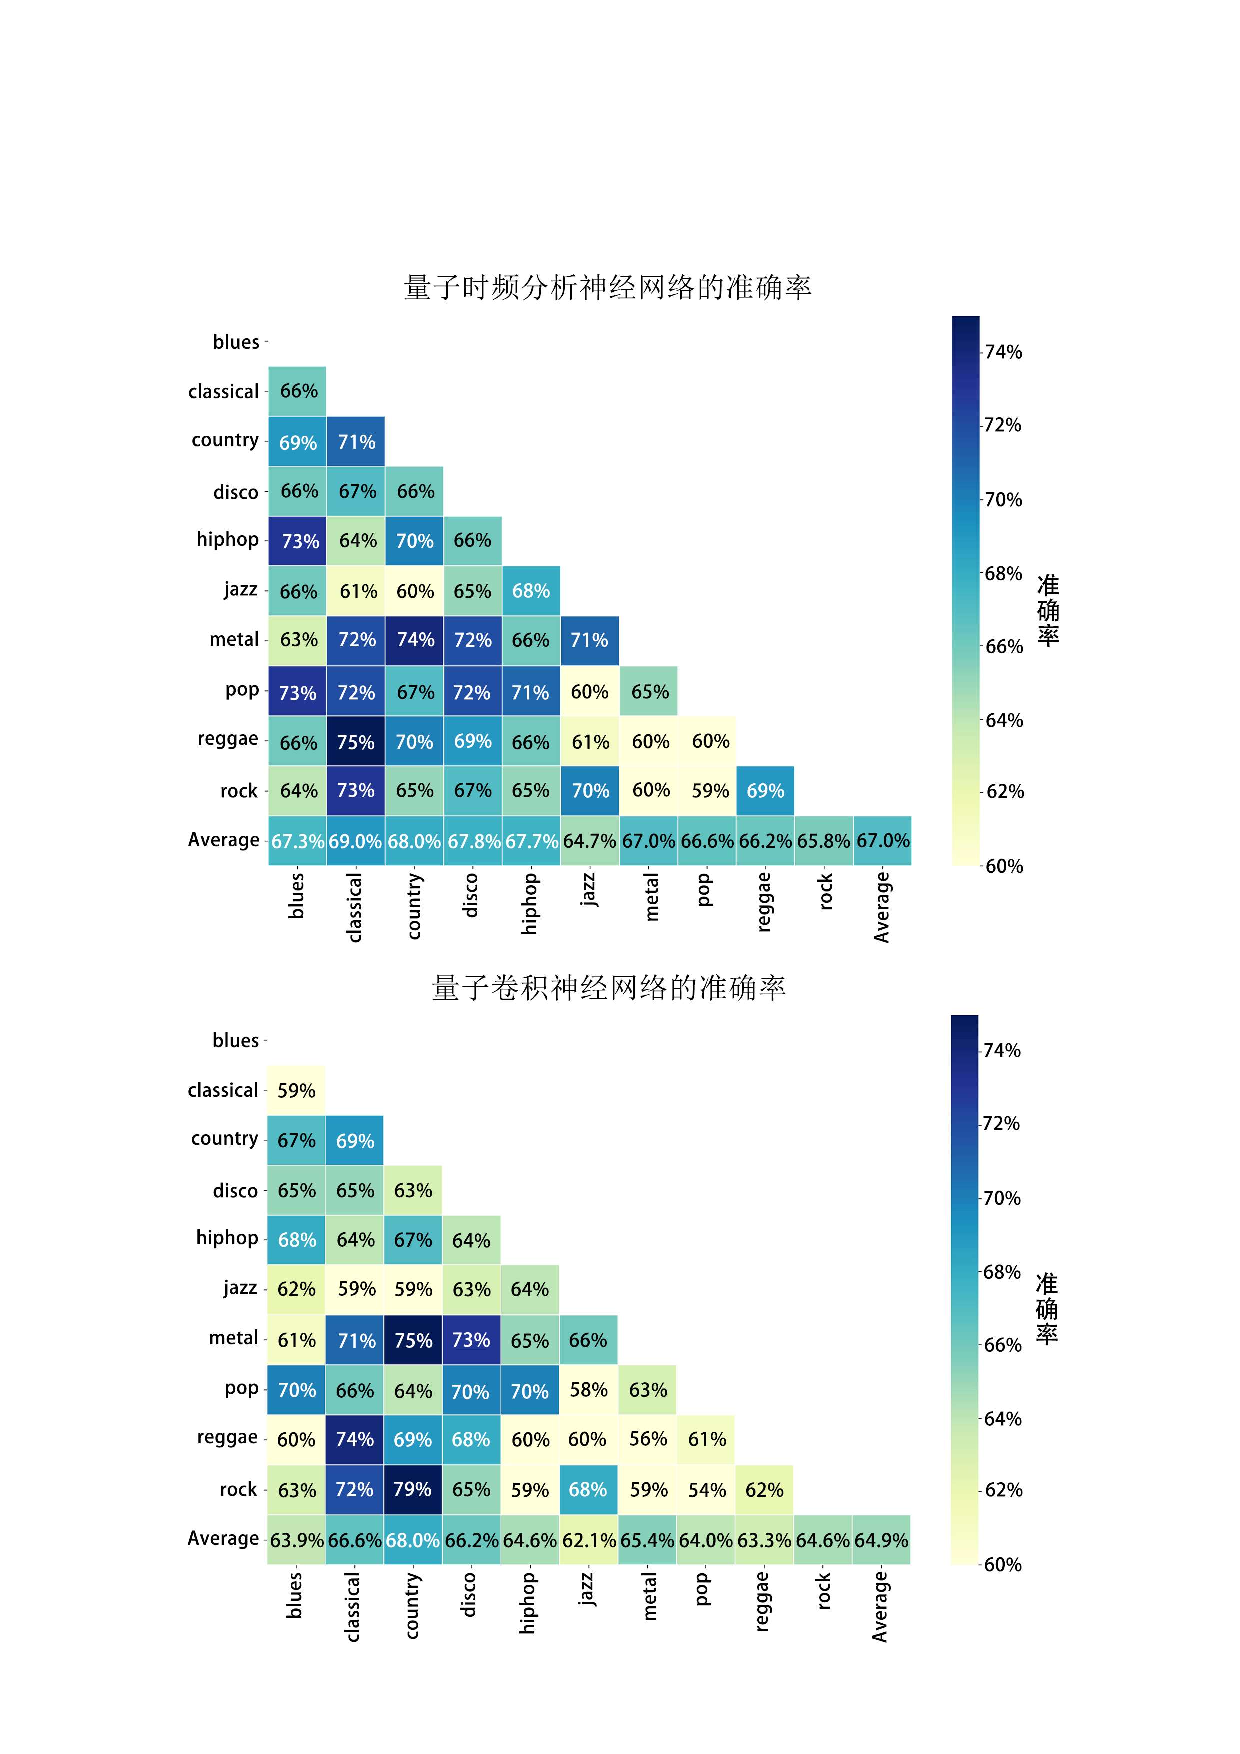
\includegraphics[width=0.6\textwidth]{images/The accuracy of QANN and QCNN.pdf}
	\caption{量子时频分析神经网络与量子卷积神经网络分类准确率对比}
	\label{fig:The accuracy of QANN and QCNN}
\end{figure}

除了纯粹的分类效能，在NISQ设备的工程落地层面，算法复杂度与部署成本同样是核心考量指标。结合表~\ref{tab:qann_vs_qcnn} 的量化汇总可知，在参数效率方面，量子卷积神经网络的参数量需要随架构搜索在 6 至 30 之间动态变动；虽然其在最优配置下报告了 79.47\% 的单点准确率，但这需要投入庞大的搜索开销。相比之下，量子时频分析神经网络采用固定的分层网络结构，仅需 33 个可训练参数即可使最佳准确率稳定在 75$\pm$1.0\%。这种无需架构搜索的设计，不仅大幅降低了经典计算开销和量子线路编译成本，同时在实验复现性与部署便利性上展现出明显优势，赋予了该模型在同等条件下更优的成本效益。

\begin{table}[!htb]
	\vspace{5pt}
	\renewcommand{\arraystretch}{1.2}
	\centering
	\caption{量子时频分析神经网络与量子卷积神经网络的方法比较分析}
	\label{tab:qann_vs_qcnn}
	\begin{tabular}{@{}lll@{}}
		\toprule
		\textbf{比较维度} & \textbf{量子时频分析神经网络} & \textbf{量子卷积神经网络}\citess{cong2019quantum} \\
		\midrule
		训练稳定性 & 75$\pm$1.0\% (经验证) & 79.47\% (单次结果) \\
		参数量 & 33 (固定) & 30 (需搜索) \\
		架构搜索 & 无需搜索 & 需进行搜索 \\
		部署复杂度 & 简单 & 复杂 \\
		计算成本 & 低 (无搜索) & 高 (搜索+训练) \\
		编码创新性 & 量子时序编码特定设计 & 传统角度/振幅 \\
		特征处理 & MFCC时频特征 & MFCC统计特征 \\
		NISQ适用性 & 高 & 中 \\
		成本效益 & 更优 & 较低 \\
		\bottomrule
	\end{tabular}
\end{table}



（4）与经典卷积神经网络的对比

为验证模型在极低参数限制下的特征表达能力，本文将量子时频分析神经网络与参数规模相同（仅 33 个参数）的经典CNN进行了对比。该33参数经典CNN的具体网络拓扑如下：输入为与量子模型相同的 $16 \times 13$ 维MFCC时频特征图（16帧×13维MFCC系数），网络由两个卷积层构成特征提取主体。第一层卷积采用 $3 \times 3$ 卷积核（含偏置），输入通道数为1、输出通道数为1，共 $3\times3\times1\times1+1=10$ 个参数；紧跟批归一化层（2个参数）和 $2\times2$ 最大池化层。第二层卷积同样采用 $3\times3$ 卷积核（不含偏置），输入通道数为1、输出通道数为1，共 $3\times3\times1\times1=9$ 个参数；随后经批归一化层（2个参数）和自适应平均池化层压缩至 $2\times2$ 的空间尺寸。最终将池化后的4维特征展平，经全连接层映射至二分类输出（$4\times2+2=10$ 个参数），参数合计 $10+2+9+2+10=33$。该设计在33参数约束下尽可能压缩了卷积通道数与全连接层神经元数，同时通过批归一化稳定浅层网络的训练过程、以自适应平均池化实现灵活的空间降维，确保对比实验的公平性。图~\ref{fig:performance_curves_comparison} 记录了模型在准确率、精确率、召回率和 F1 分数四个关键指标上的全周期训练轨迹。首先从准确率曲线可以观察到，在训练初期的前 20 个迭代步内，量子网络的测试准确率上升梯度明显高于经典 CNN，并迅速拉开性能差距。这一现象表明，在同等稀疏参数的严格限制下，量子时频分析神经网络能够更高效地探索特征流形。其内在机制在于利用高维希尔伯特空间的量子叠加态映射，以更小的参数代价捕获了音频信号的核心声学纹理。至收敛后期，量子网络的测试准确率平稳收敛于 75\% 附近，而经典 CNN 的表征瓶颈凸显，准确率停滞在 70\% 左右。

\begin{figure}[!htb]
	\centering
	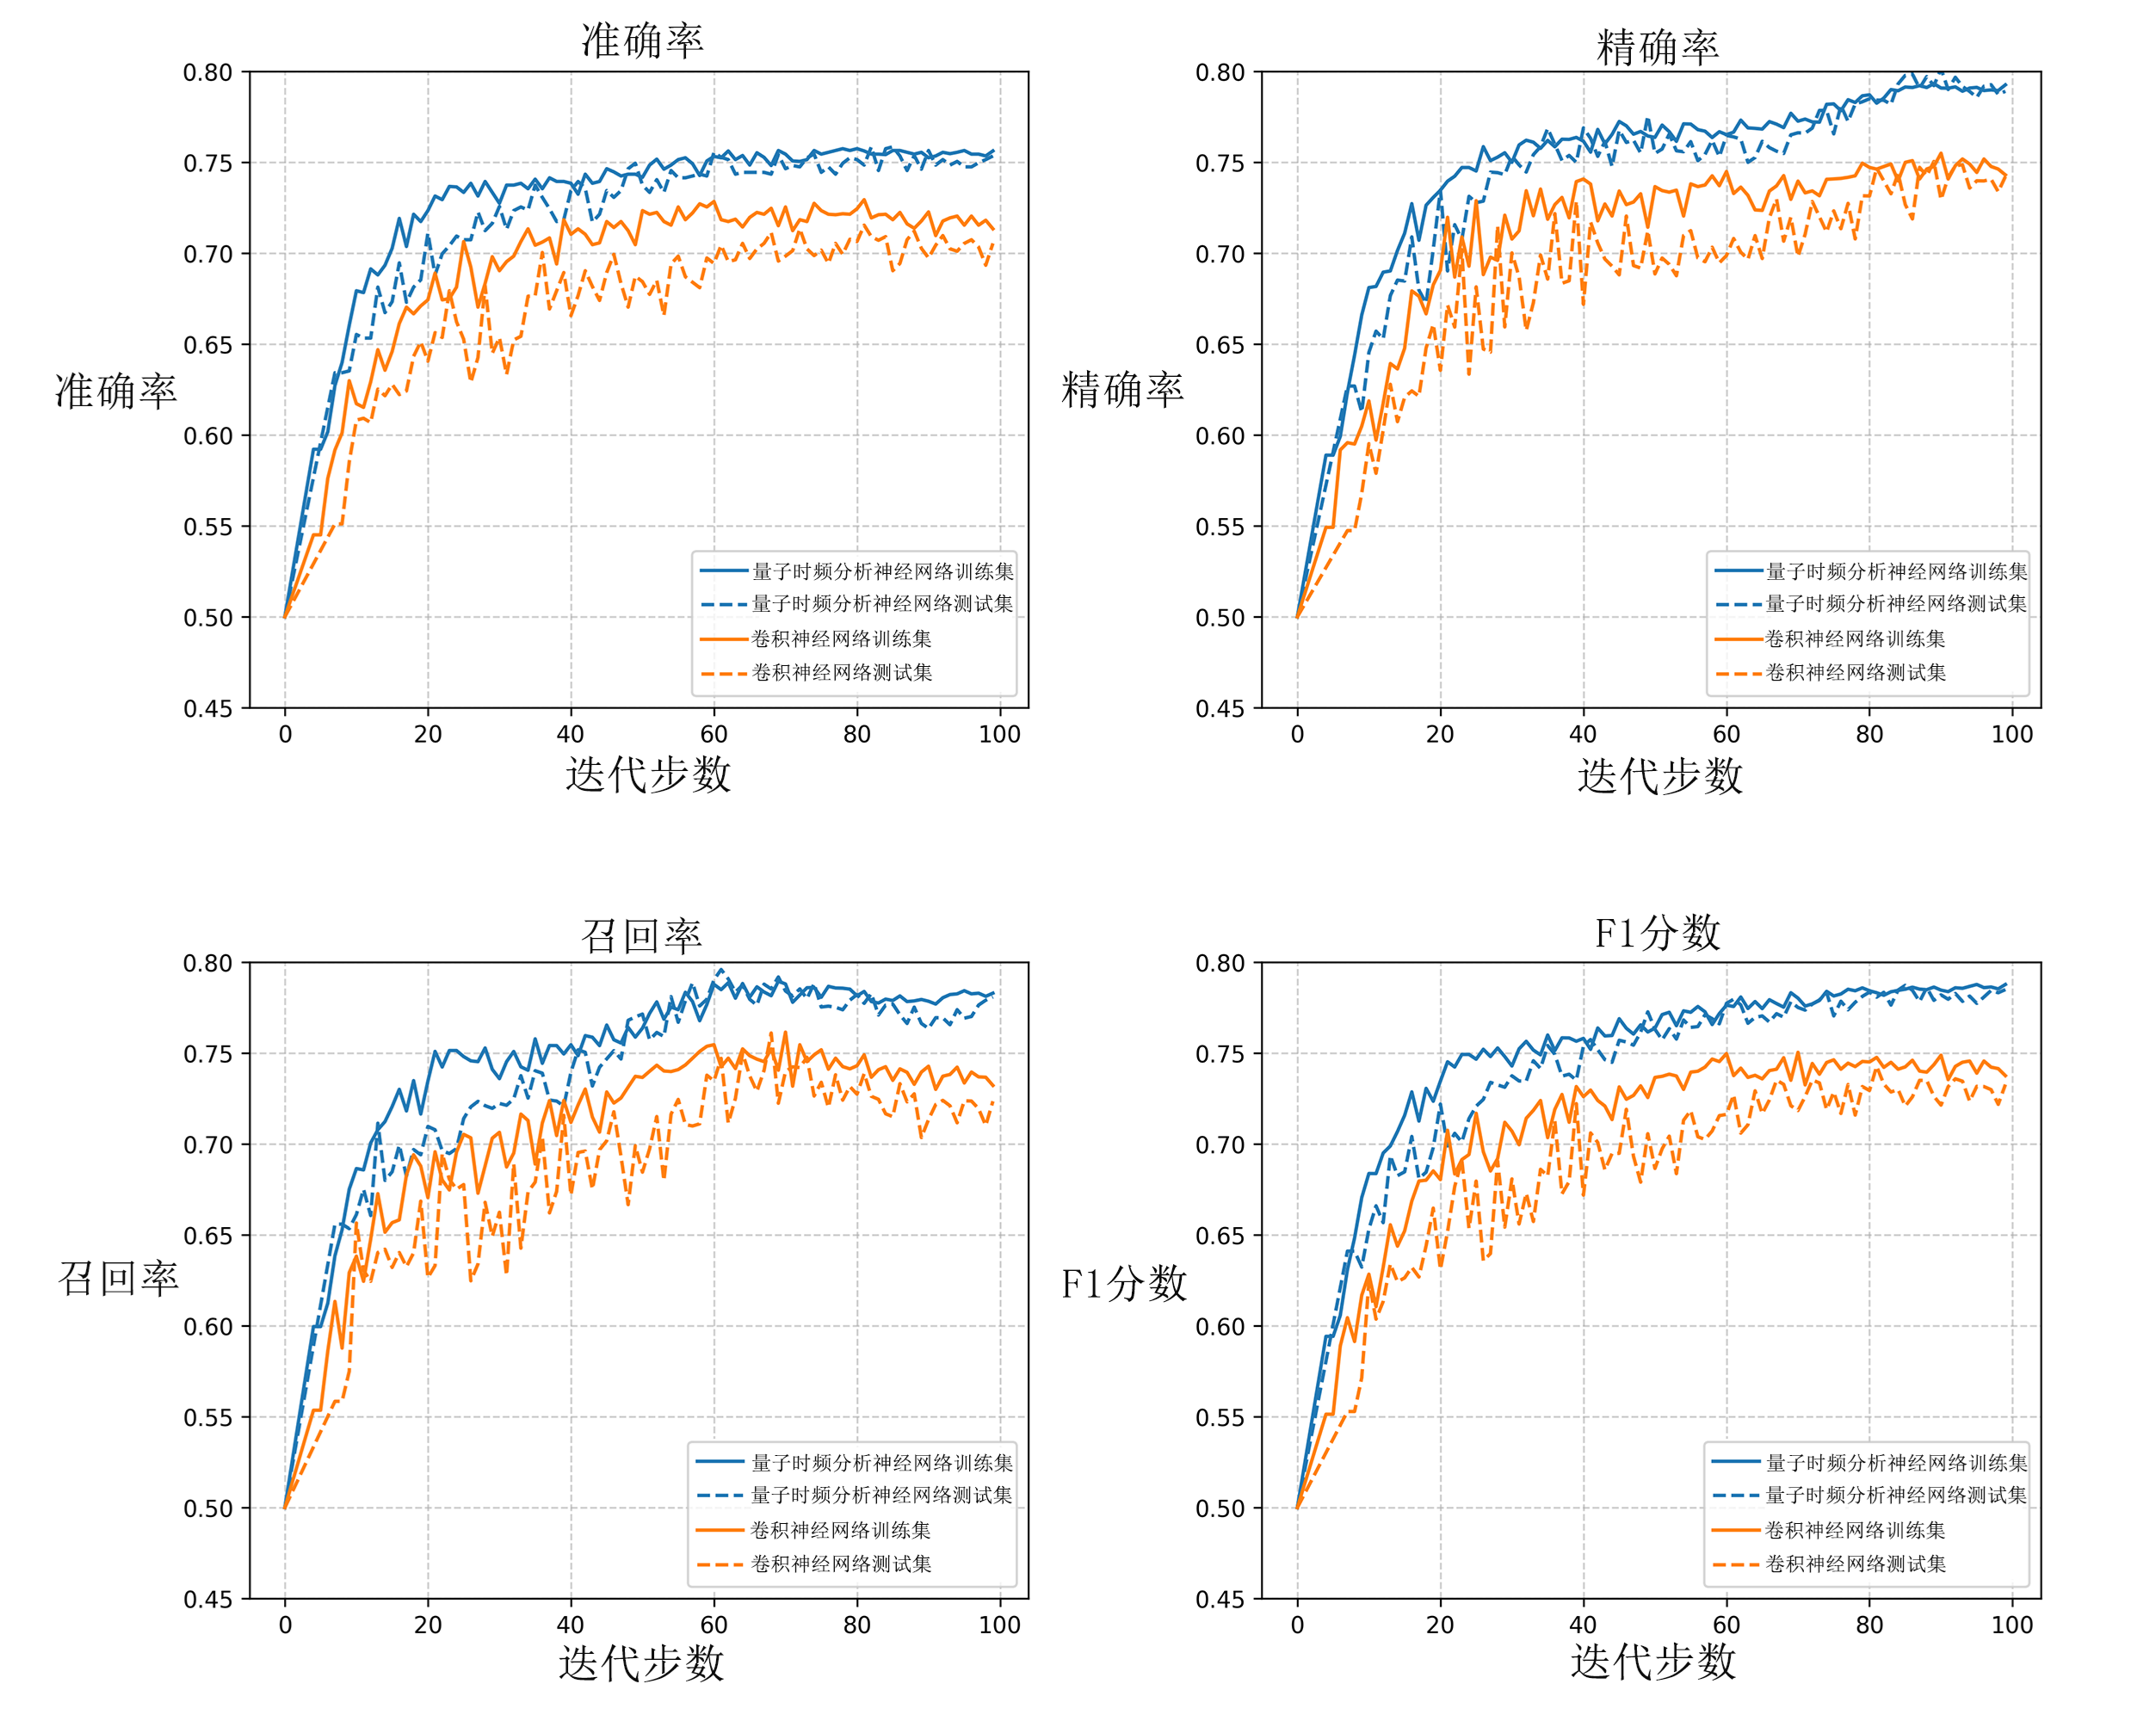
\includegraphics[width=1\textwidth]{images/performance_curves_comparison.png}
	\caption{量子时频分析神经网络与经典 CNN 基线模型的分类性能指标对比}
	\label{fig:performance_curves_comparison}
\end{figure}

进一步分析精确率与召回率的动态演化可以发现，经典 CNN 在 40 至 80 步区间出现了较大幅度的锯齿状波动，说明浅层经典网络在面对非平稳声学特征时，其分类决策边界极易受到批次样本方差的干扰。相比之下，量子网络的精确率与召回率曲线更为平滑，且均平稳收敛至 0.78 左右，证实了参数化量子滤波器中的双比特纠缠门通过建立相邻时频特征间的强关联，有效提升了决策边界的鲁棒性。此外，在反映模型综合辨识水平的 F1 分数上，量子网络在全周期内均保持领先，表明其在捕获长程时序依赖方面具备明显优势，成功避免了在特定相似流派上的性能坍塌。

最后，从模型泛化能力的角度考察各子图中训练集与测试集的走势间隙。经典 CNN 在训练后期，其测试集指标方差明显增大，显现出典型的小样本过拟合趋势；反观量子时频分析神经网络，其训练与测试曲线在整个演化周期内高度贴合，泛化间隙被有效抑制。这种优异的抗过拟合能力主要源于量子结构固有的物理正则化效应：演化线路中酉变换的保范性以及量子滤波器内深度的参数共享机制，从结构层面上对假设空间进行了严格约束，从而在极低参数规模下实现了更可靠的声学特征泛化。


\subsubsection{时序编码能力验证与结构敏感性分析}

\label{subsec:validation_and_ablation}

为定量验证量子时序编码在高维希尔伯特空间中保留音频时序信息的能力，本节引入了时间滞后敏感性评估机制——通过计算不同时序扰动条件下量子态之间的保真度差值，度量模型对时间维度的感知程度。

如图~\ref{fig:Temporal encoding capability} 的箱线图所示，实验系统对比了“反转距离”（即将音频帧的全局时序完全逆转后产生的量子态差异）与“扰动距离”（即在局部时间窗口内进行微小随机平移产生的量子态差异）。数据分布表明，反转距离的中位数约为 1.8，且由于存在较大的结构性偏移，其整体分布区间明显拉长（最大值超过 8.0），使得平均反转距离达到了 2.106。这一巨大的状态偏移有力地证明了：量子时序编码对音频信号的全局宏观时间顺序具有高度的敏感性。由于时间索引被严格映射为相互正交的量子基态，任何破坏全局时序的操作都会导致量子态在投影空间中发生剧烈偏离。

\begin{figure}[!htb]
	\centering
	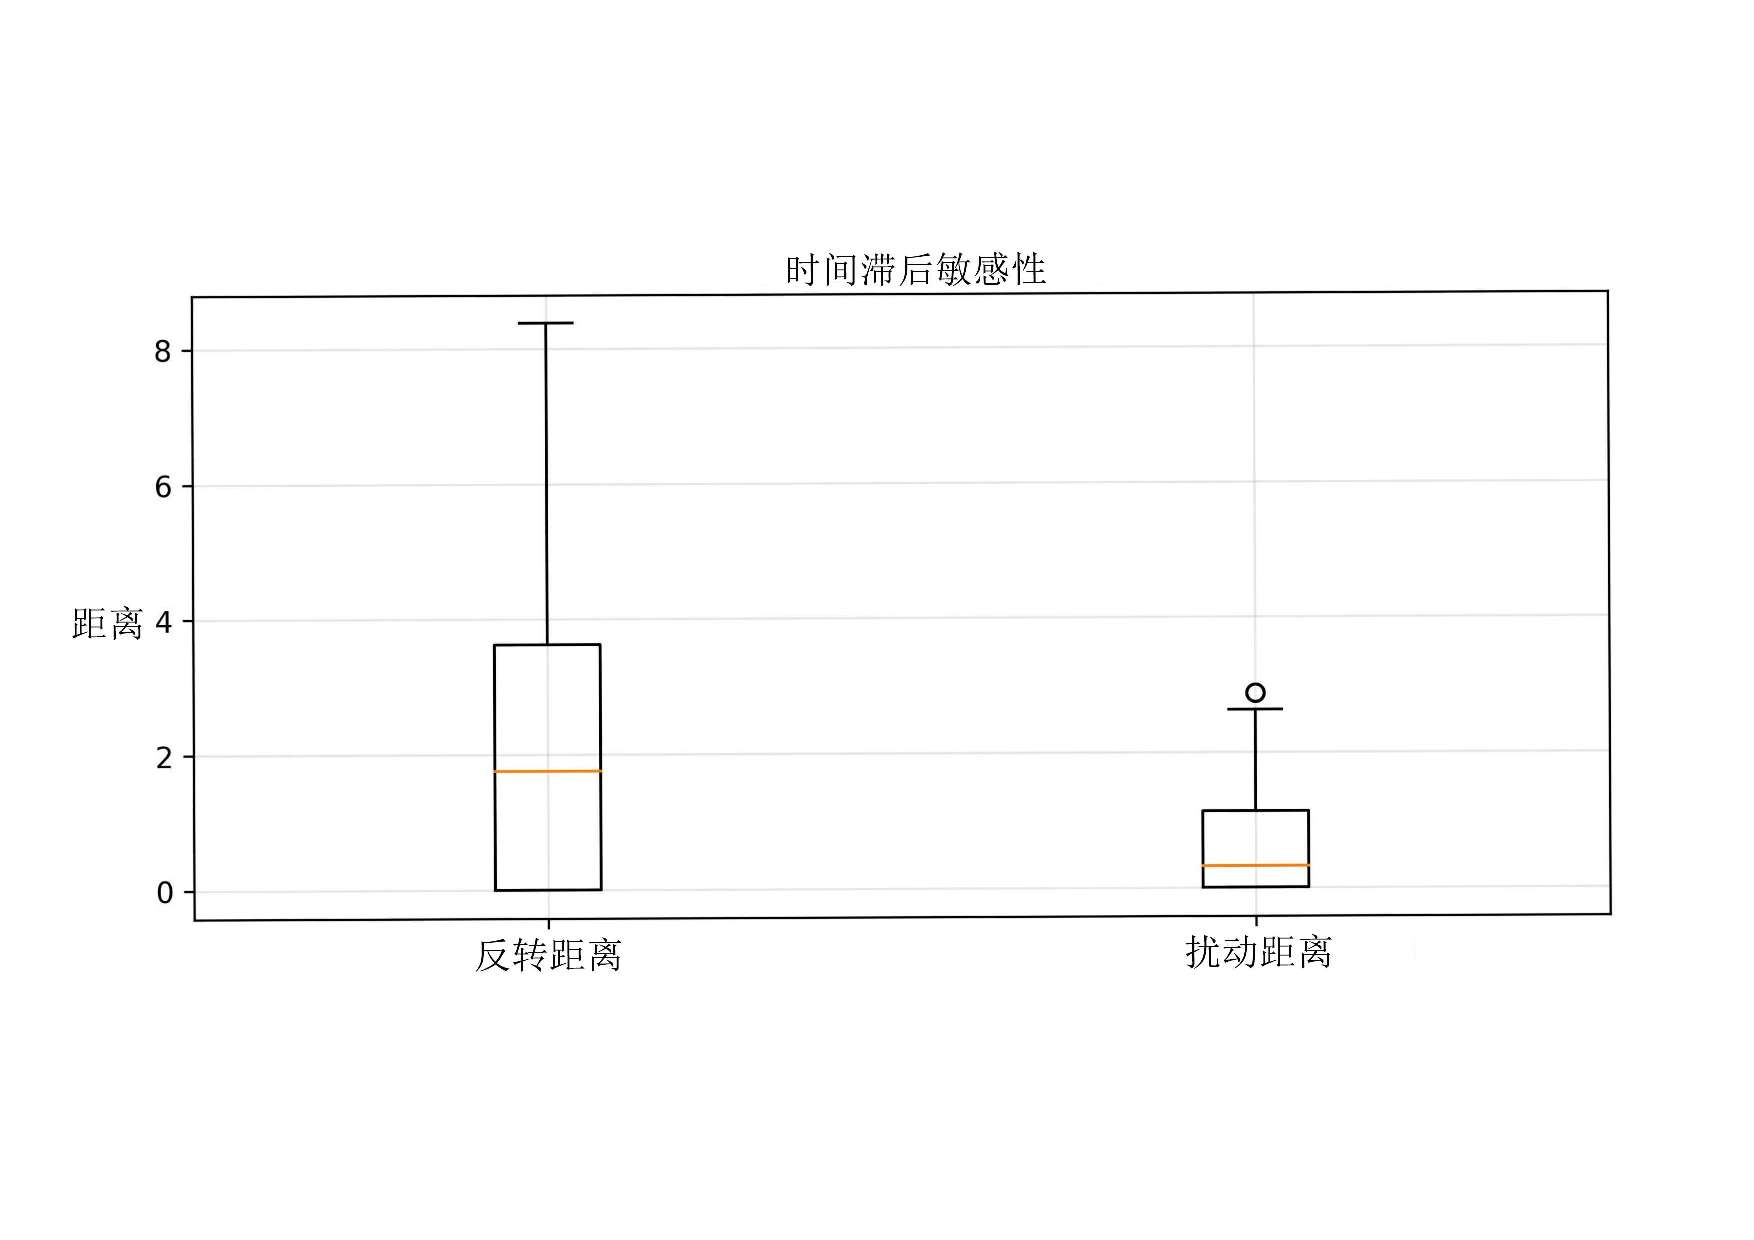
\includegraphics[width=1.0\textwidth]{images/temporal_lag_sensitivity.pdf}
	\caption{量子时序编码能力的定量验证}
	\label{fig:Temporal encoding capability}
\end{figure}

与此同时，扰动距离的中位数仅位于 0.3 左右，且数据分布高度集中，这表明该编码方案在面对局部的微小时间抖动时能够保持良好的鲁棒性。结合实验测得的 0.531 的自相关衰减率，可以得出结论：量子时序编码不仅能够精准锚定全局时间坐标，还能将相邻时间帧有效地关联起来，形成连贯且抗噪的局部声学上下文。

此外，为了深入探究量子时频分析神经网络中核心网络架构的设计必要性及其对整体分类性能的影响，本文进行了结构敏感性分析。在此实验中，我们将网络量子卷积层中精心设计的参数化量子滤波器（由 U3 旋转门与 Ising 族纠缠门构成）替换为最基础的、无参数的纯 CNOT 门结构，以观察特征提取器表达能力的退化情况。

如图~\ref{fig:CNOT comparison} 所示，采用纯 CNOT 基准卷积层的模型在训练动力学和最终收敛精度上均暴露出明显的劣势。从训练轨迹来看，在迭代的前 30 步内，测试集的准确率和损失函数均出现了极其剧烈的震荡现象（准确率在 0.50 至 0.70 之间大幅波动）。这种不稳定的优化景观表明，固定相位的 CNOT 门虽然能在时间与音色特征之间建立硬性纠缠，但缺乏平滑的参数化梯度空间，导致经典优化器（如 Adam）难以在复杂的声学特征流形中找到稳定的下降路径。从最终的收敛结果来看，基于 CNOT 的模型准确率在 40 步后陷入局部最优，仅能勉强收敛至约 68\%，测试损失也停滞在 0.625 左右的高位。相比之下，本文提出的参数化滤波器架构能够稳定达到 75\% 的高准确率。这一明显的性能鸿沟充分证明：具备连续旋转自由度和可调局部纠缠能力的参数化量子滤波器，对于捕获复杂且非平稳的音频时频模式是不可或缺的。

\begin{figure}[!htb]
	\centering
	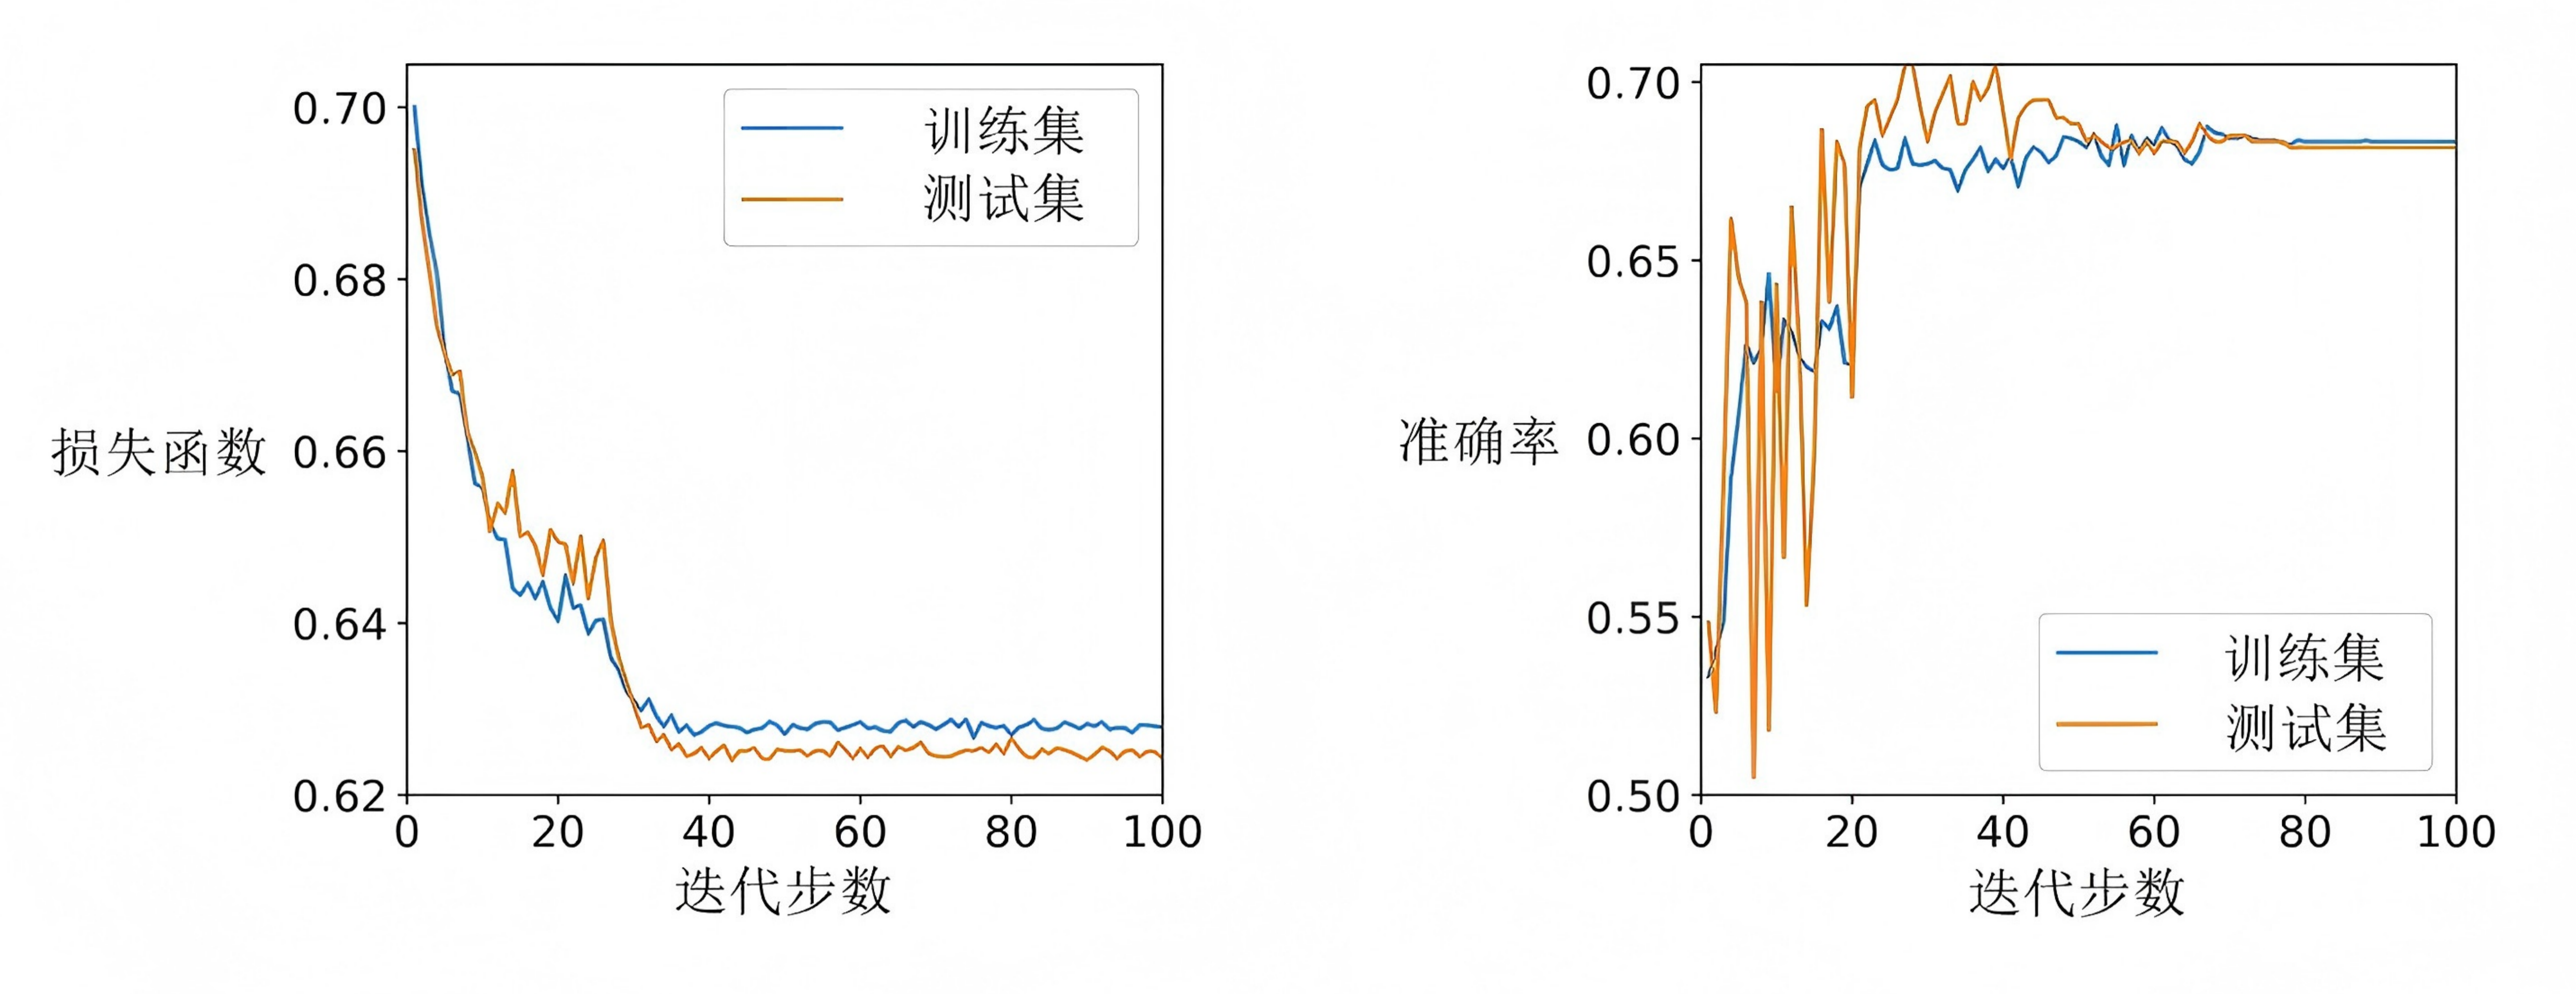
\includegraphics[width=1.0\textwidth]{images/CNOT_comparison.png}
	\caption{CNOT 基准模型的准确率与损失收敛曲线}
	\label{fig:CNOT comparison}
\end{figure}

\subsection{本章小结}
\label{sec:chapter_summary}

本章围绕基于时序编码的量子时频分析神经网络展开了论述与实验验证。在编码层面，针对已有量子音频表示方法无法保留时间信息的缺陷，本文提出了一种基于双量子比特序列纠缠的量子时序编码方案，以 MFCC 为音色特征，通过优化的量子比特复用策略将状态制备的时间复杂度控制在 $O\left(q n 2^n\right)$。在此编码之上，搭建了包含量子卷积层、池化层与全连接层的端到端量子时频分析神经网络。实验结果表明，该网络在 GTZAN 基准数据集上的分类准确率达到 75\%，优于振幅编码与角度编码。与量子卷积神经网络及同参数规模的经典 CNN 对比后发现，量子时频分析神经网络仅使用 33 个可训练参数即可取得更高的训练稳定性和泛化能力，说明该模型在 NISQ 条件下具有可行的工程部署价值。